% Author Anpassen
\newcommand{\myAuthorName}{Luis Meier}
% Titel der Arbeit anpassen
\newcommand{\myTitle}{Einsatz von ROS Industrial in einem Industrie 4.0 Demonstrator}
%%% Dokumenteinstellungen %%%
%!TEX root = doc.tex
\documentclass[
german,
	10pt, 							% The default document font size, options: 10pt, 11pt, 12pt
	%oneside, 						% Auskommentieren für einseitige Dokumentstruktur
	singlespacing,					% Zeilenabstand - Alternativen: onehalfspacing or doublespacing
	%nolistspacing, 				% Falls onehalfspacing oder doublespacing Auskomentieren!
	%parskip, 						% Auskommentieren für Einzug nach Absatz
	headsepline, 					% Linie unter Kopfzeile
]{scrbook} 							% The class file specifying the document structure


% ====================================================================
% ==						 Packages								==
% ====================================================================
%%% Dokumentinformationen %%%
\usepackage[
	pdftitle={\myTitle},			% Pdf-Titel
	pdfsubject={},
	pdfauthor={\myAuthorName},		% Author
	pdfkeywords={},	
	hidelinks						% Links nicht einrahmen
]{hyperref}

%%% Standard Packages %%%
\usepackage[utf8]{inputenc}
\usepackage[T1]{fontenc}
\usepackage{graphicx, subfigure}	% Einbinden von Grafiken mit \includegraphics
\usepackage{wrapfig}				% Einbinden von Grafiken mit 
\usepackage{lmodern}
\usepackage{color}					% Für Farben z.B. in Tabellen
\usepackage{transparent}			% Für transparente Farben
\usepackage{colortbl}				% für Farben in Tabellen z.B. mit \rowcolor{Gray}
\usepackage{blindtext}				% für Beispieltexte
\usepackage{float}					% Für [H] --> Hier Befehl für Grafiken und Tabellen usw.
\usepackage{geometry}				% Benötigt für Ränder	
%\usepackage[nswissgerman]{babel}
\usepackage[ngerman]{babel}

\usepackage[
	acronym,
	footnote,
	toc,
	section,
	nopostdot,
	nonumberlist
]{glossaries}

%%% Math Packages %%%
\usepackage{amsfonts}				% zusätzliche Schriftzeichen der American Mathematical Society
\usepackage{amsmath}				% mathematische darstellung gem AMS
\usepackage{amssymb} 				% mathematische Symbole aus AMS
\DeclareMathSymbol{*}{\mathbin}{symbols}{"01} % Punkt statt stern bei Multiplikationen

%%% Usefull Packages %%%
\usepackage{url}					% Einbinden von URL's in Text
\usepackage[squaren]{SIunits}		% Zur benutzung von SI-Einheiten
\usepackage{longtable}				% Ermöglicht Tabellen über mehrere Seiten
\usepackage[table,dvipsnames]{xcolor}
							% Für Glossar und Nomenkaltur (evtl ersetzen mit Glossary-Package)
\usepackage{enumitem}				% Zur auflistung mit Zahlen statt punkten

%%% Styling Packages %%%
\usepackage{colortbl}				% Farben in Tabellen
\usepackage{tabularx}				% Bessere Darstellung von Tabellen mit \tabularx
\usepackage{array}					% Benötigt von tabularx
\usepackage[absolute]{textpos}		% Absolute Text Positionierung
\usepackage{scrlayer-scrpage}		% Für Headed/Footer
\usepackage{textcomp}				% Für div Zeichen z.B. Copyright
%\usepackage[scaled]{arial}			% Arial Font

%%% Plots, Mindmaps etc %%%
%\usepackage{tikz}
%\usetikzlibrary{mindmap}


%%% Import Coding %%%
\definecolor{BGgray}{gray}{0.95}	%Hintergrundfarbe für code
\usepackage[newfloat]{minted}
\setminted{
	breaklines=true,				% Automatic Line Breaking
	frame=lines,					% Lines on top and Bottom of Frame
	framesep=1mm,					% Frame Separation 
	baselinestretch=1.1,			% Interlining of the code
	bgcolor=BGgray,					% Sets background color
	fontsize=\footnotesize,			% Sets Fontsize
	%linenos=true,					% Enables Line Numbers
	%showspaces=true,				% Enables sign for spaces
	obeytabs=false,
	tabsize=2,
}
\usemintedstyle{default}
%%% Definition des Verzeichnisses für den Code
\usepackage{listings}
\renewcommand{\lstlistingname}{Sourcecode}
\renewcommand{\lstlistlistingname}{\lstlistingname verzeichniss}

%%% ZHAW Titelpage %%%
\usepackage{wallpaper} 				% Bild hinter Text laden

%%% Index und Referenzen %%%
\usepackage[super,square]{natbib}	% für BibTeX Literaturverzeichnis
\usepackage{makeidx}				% Benötigt für Index

%%% PDF-Import %%%
\usepackage{pdflscape}				% Drehen von PDF's
\usepackage{pdfpages}				% Einzelne PDF-Seiten importieren

% ====================================================================
% ==						Document Styling						==
% ====================================================================

%%% Definition des Textbereichs %%%
\geometry{
	a4paper,
	top=30mm,
	left=30mm,
	right=30mm,
	bottom=30mm,
	headsep=10mm,
	footskip=10mm
}

%%% Definition der Textposition %%%
\setlength{\TPHorizModule}{30mm}
\setlength{\TPVertModule}{\TPHorizModule}
\textblockorigin{10mm}{10mm} 		% start everything near the top-left corner
\setlength{\parindent}{0pt}

%%%% Horizontale Linien auf Titelseite %%%
\newcommand{\HRule}{\rule{\linewidth}{0.5mm}}

%reference to source items inlc source number
\newcommand{\srcref}[1]{\nameref{src:#1} \cite{#1}}

%%% Kopf- und Fußzeile %%%
%\lohead{\myAuthorNames}
\rohead{\myTitle}
\pagestyle{scrheadings}

%%% Quellverzeichnis Style %%%
%\bibliographystyle{abbrv}
\bibliographystyle{ieeetr}

%%% Definition von Farben %%%
\definecolor{gray}{rgb}{0.95,0.95,0.95}
\definecolor{darkgray}{rgb}{0.4,0.4,0.4}

% ====================================================================
% ==				Sonstige Einstellungen							==
% ====================================================================
%%% Besondere Trennungen %%%
\hyphenation{De-zi-mal-tren-nung}

%%% Pfad für Bilder %%%
\graphicspath{{images/}}				% Gibt Pfad für Bilder an
%%% Neue Fig bennenung %%%
\numberwithin{figure}{chapter}

%%% Abb. statt Abbildung %%%
\addto\captionsngerman{
	\renewcommand{\figurename}{Abb.}
	\renewcommand{\tablename}{Tab.}
}		% Hier müssen einige Sachen Personalisiert werden!

\usepackage{dirtree}

%%% Aufsetzen des Glossars %%%
\makeglossaries
%!TEX root = ../doc.tex
\chapter*{Glossar}
\label{sec:Glossar}
\addcontentsline{toc}{section}{Abkürzungsverzeichnis}\label{cha:abkürzungsverzeichnis}

In diesem Abschnitt werden Abkürzungen und Begriffe kurz erklärt.
%\setglossarystyle{altlistgroup}
\printglossary[title=]



\usepackage{blindtext}
\usepackage{caption}

\newenvironment{code}{\captionsetup{type=listing}}{}
\SetupFloatingEnvironment{listing}{name=Codesnippet}

%%% Begin des Dokuments %%%
\begin{document}

\title{\myTitle}
\author{\myAuthorName}

%%% Titel, Abstract %%%
\frontmatter
%!TEX root = ../doc.tex
\begin{titlepage}

% Logo

%
\includegraphics[scale=1]{images/logos/IMS.pdf}
\ThisTileWallPaper{\paperwidth}{\paperheight}{images/logos/IMS.pdf} % {images/logos/*.pdf}

\begin{minipage}[b]{0.117\textwidth}
\hskip 0.05cm
\end{minipage}
\begin{minipage}[b]{0.91\textwidth}
\begin{tiny}.\end{tiny}\vskip 2.8cm
	{\huge

	% Projekt Name (max. 2 Zeilen)
	\textbf{\underline{VT2}}\\
	\textbf{\underline{FS17 MSE}}\\

	% Projekt Titel (max. 4 Zeilen)
	\myTitle
	\vskip 0.5cm}

	\begin{minipage}[b]{0.27\textwidth}
	\hrule\vskip 0.5cm
		\textbf{Autor}\\
		\\
	\end{minipage}
	\begin{minipage}[b]{0.03\textwidth}
	\hskip 0.5cm
	\end{minipage}
	\begin{minipage}[b]{0.7\textwidth}
	\hrule\vskip 0.5cm
		\myAuthorName \\
		\\
	\end{minipage}

	\begin{minipage}[b]{0.27\textwidth}
	\hrule\vskip 0.5cm
		\textbf{Hauptbetreuung}\\
		\\
	\end{minipage}
	\begin{minipage}[b]{0.03\textwidth}
	\hskip 0.5cm
	\end{minipage}
	\begin{minipage}[b]{0.7\textwidth}
	\hrule\vskip 0.5cm
		Dr. Marcel Honegger\\
		\\
	\end{minipage}



	\begin{minipage}[b]{0.27\textwidth}
	\hrule\vskip 0.5cm
		\textbf{Datum}
	\end{minipage}
	\begin{minipage}[b]{0.03\textwidth}
	\hskip 0.5cm
	\end{minipage}
	\begin{minipage}[b]{0.7\textwidth}
	\hrule\vskip 0.5cm
		\today
	\end{minipage}
\end{minipage}
\vskip 0.5cm




\end{titlepage}

%!TEX root = ../doc.tex
\chapter*{Abstract}
\label{sec:Abstract}
Industrieroboter werden von diversen Herstellern angeboten, diese Roboter besitzen meist eine proprietäre Steuerung und Bahnplanung. Jeder Hersteller von Robotern und den entsprechenden Steuerungen bietet in der Regel ein sehr ähnliches Funktionspaket an. Der Aufruf dieser Funktionen und die dazu benötigte Programmiersprachen sind nicht bei allen Herstellern gleich. Bis anhin sind durch die Hersteller der Roboter keine Bestrebungen ersichtlich eine vereinheitlichte Programmiersprache und Ansteuerung der Roboter zu entwickeln.
Mit dem Robot Operating System (ROS) und der dazugehörigen Erweiterung für Industrielle Roboter (ROS-Industrial) ist ein Framework vorhanden, welches es ermöglicht universell Software und Applikationen in der Robotik zu entwickeln. \\

Ziel dieser Arbeit ist es die Möglichkeiten und Einschränkungen von ROS-Industrial zu ermitteln, dazu soll eine Entwicklungsumgebung mit ROS-Industrial aufgesetzt werden und anschliessend eine Montageaufgabe mit ROS-Inudstrial realisiert werden. Als Montageaufgabe ist das Zusammenbauen eines Kugelschreibers, im Industie 4.0 Demonstrator vorgesehen. Der Industrie 4.0 Demonstrator ist ein Projekt der ZHAW und diverser Industriepartner. Es soll die vielen Aspekte von Industrie 4.0 in einem einzelnen Demonstrator veranschaulichen. Die Montageaufgabe soll auf den drei Robotern ABB IRB120, Stäubli TX2-60l und Universal UR3 realisiert werden.\\

Resultat dieser Arbeit ist eine fertig Aufgesetzte Arbeitsumgebung für ROS und ROS-Industrial, und eine Implementierung der Montage Aufgabe in den Industrie 4.0 Demonstrator. Es konnten jedoch nicht alle in der Aufgabenstellung geforderten Ziele erreicht werden. Hauptgründe dafür sind ein noch nicht angelieferter Roboter von Stäubli, Komplikationen bei der Ansteuerung der SMC Aktuatoren über EtherCAT und falsch bestellte Teile. Diese Komplikationen verhinderten, dass die implementierte Montageaufgabe vollständig geprüft und verbessert werden konnte. \\

Die Möglichkeiten von ROS-Industrial sind extrem Umfangreich, es werden durch die Open Source Community eine Vielzahl an Paketen mit Funktionen angeboten. Diese ermöglichen es in sehr kurzer Zeit eine sehr Komplexe Aufgabe zu lösen. 
Die Open Source Community ist zugleich aber auch ein Grund für diverse Einschränkungen von ROS und ROS-Industrial. Da viele Pakete nicht oder nur schlecht gewartet werden kommt es oft vor, dass nicht vollständig funktionsfähige Pakete implementiert werden müssen und diese allenfalls gepatcht werden müssen. Es kann zudem auch vorkommen, dass Nodes aufgrund von nicht nachvollziehbaren Gründen neu gestartet werden müssen.

%!TEX root = ../doc.tex

\chapter*{Vorwort}
\label{sec:Vorwort}
Die Robotik faszinierte mich, seit ich das erste mal mit ihr in Kontakt kam. Ich konnte jedoch noch nie ein Projekt mit einem Industrieroboter miterleben. Das Thema ROS, ein so umfangreiches Softwareprojekt und C++ waren für mich absolutes Neuland und stellten mich oft vor grosse Herausforderungen. Einigie dieser Herausforderungen kosteten mich viele Nerven, mit ein paar wenigen bin ich bis zum Schluss nicht klar gekommen. \\
\\



\cleardoublepage

%% Eigenständigkeitserklärung - Entsprechendes auskommentieren
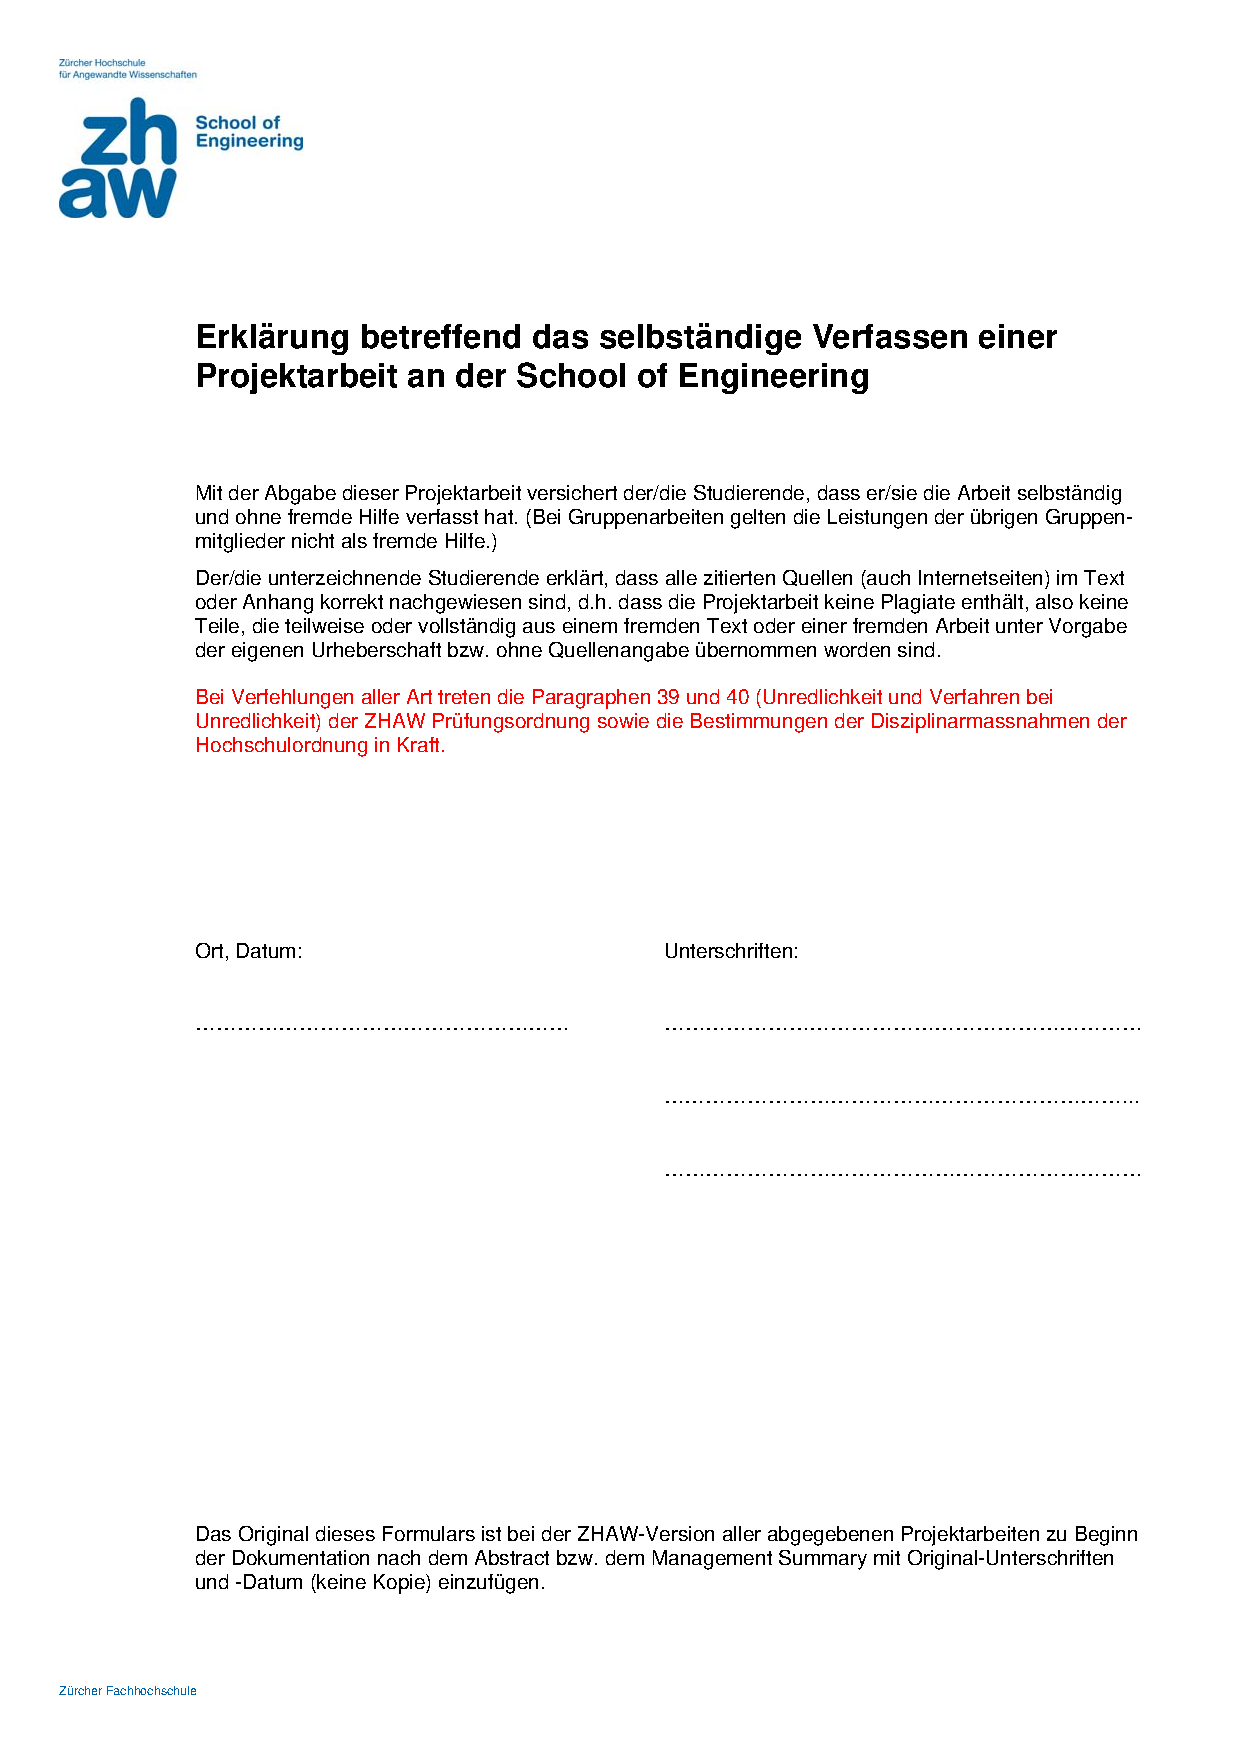
\includepdf[pagecommand={\thispagestyle{plain}}]{images/Erklaerung_PA.pdf} 
%
\includepdf[pagecommand={\thispagestyle{plain}}]{images/Erklaerung_BA.pdf}

\tableofcontents		% Inhaltsverzeichnis

\chapter{Verzeichnisse}
\printglossary[type=\acronymtype,title={Abkürzungen}]
\printglossary[title=Glossar]
%%% Abbildungsverzeichnis %%%
\listoffigures
\addcontentsline{toc}{section}{Abbildungsverzeichnis}
%%% Tabellenverzeichnis %%%
\listoftables
\addcontentsline{toc}{section}{Tabellenverzeichnis}%%!TEX root = ../doc.tex
\chapter*{Glossar}
\label{sec:Glossar}
\addcontentsline{toc}{section}{Abkürzungsverzeichnis}\label{cha:abkürzungsverzeichnis}

In diesem Abschnitt werden Abkürzungen und Begriffe kurz erklärt.
%\setglossarystyle{altlistgroup}
\printglossary[title=]

%%% Sourcecodeverzeichnis %%%
\lstlistoflistings
\addcontentsline{toc}{section}{Codesnippetsverzeichnis}

\mainmatter


%%% Hauptteil %%%
%!TEX root = ../doc.tex
\chapter{Einleitung}
\label{sec:Einleitung}
Industrieroboter, wie sie von diversen Herstellern angeboten werden besitzen meistens eine proprietäre Steuerung. Die Hersteller dieser Steuerungen bieten meistens ein sehr ähnliches Funktionspaket an, jedoch wird über die Hersteller hinweg keine einheitliche Programmiersprache verwendet, es gibt zum Beispiel RAPID bei ABB, oder KRL bei KUKA. Bis anhin sind durch die Roboterhersteller keine Bestrebungen zu einer einheitlichen Programmiersprache in Sicht. \\
Mit dem Robot Operating System (ROS) ist ein Framework vorhanden, welches sich für die Entwicklung von universeller Software für Roboter anbietet. ROS wurde ursprünglich für den Teilbereich der Mobilrobotik entwickelt. Durch die Erweiterung ROS-Industrial steht jedoch ein weiteres Framework zur Verfügung, welches die Fähigkeiten von ROS auf die Anforderungen in der Industrie erweitert. 


\section{Ausgangslage}
\label{sec:Ausgangslage}
Im Rahmen zweier Bachelorarbeiten wurde im Frühlingssemester 2017 ein Industrie 4.0 Demonstrator konzeptioniert und entwickelt, welcher die diversen Aspekte von Industrie 4.0 aufzeigen können soll. Dazu können Kugelschreiber durch den Kunden - respektive den Messebesucher - in verschiedenen Zusammenstellungen konfiguriert werden, anschliessend werden diese Kugelschreiber durch den Demonstrator zusammengebaut. \\
Der Demonstrator wird in Zusammenarbeit mit mehreren Industriepartnern realisiert, die Industriepartner stellen diverse Komponenten für den Industrie Demonstrator zur Verfügung.

\subsection{Projektorganisation}
Das gesamte Projekt Industrie 4.0 Demonstrator wird durch mehrere Personen mit unterschiedlichen Zuständigkeiten realisiert. Die Planung des mechanischen Aufbaus der Anlage wird durch die beiden Bachelorstudenten Andrin Meister und Christian Hartmann durchgeführt. Claude Hasler entwickelt im Rahmen einer Verteifungsarbeit einen Minideltarobtoer, welcher für das Feeden der Kleinteile Zuständig ist.

\section{Aufgabenstellung}
\label{sec:Aufgabenstellung}
Im Rahmen dieser VT2 soll eine konkrete Montageaufgabe für den Industrie 4.0 Demonstrator (SmartPro) mit einem Stäubli Industrieroboter realisiert werden, wobei als Programmiersprache \verb!C++! und das ROS Industrial Framework eingesetzt werden. Nach Möglichkeit soll aber keine Stäubli spezifische Software entwickelt werden. Die Portierbarkeit dieser Anwendung soll schliesslich mit einem Wechsel des gewählten Roboters zu einem Universal Robots UR3 - respektive einem ABB IRB120 - gezeigt werden.\\
Dazu wurden folgende Arbeitspakete definiert:
\begin{itemize}
	\item Aufsetzen einer Entwicklungsumgebung mit ROS Industrial.
	\item Simulation einer einfachen Montageaufgabe des Industrie 4.0 Demonstrators, wobei als Roboter ein Stäubli Industrieroboter, ein Universal Robots UR3 und ein ABB IRB120 verwendet werden sollen.
	\item Entwicklung und Umsetzung der Montageaufgabe mit dem Stäubli Industrieroboter.
	\item Portierung dieser Montageaufgabe auf einen Universal Robots UR3, inklusive Vergleichstest mit dem Stäubli Roboter.
	\item Evaluation von ROS Industrial, mit einer Beurteilung dessen Möglichkeiten und Einschränkungen für industrielle Anwendungen.	 
\end{itemize}

\section{Verwendete Software}
\label{sec:VerwendeteSoftware}
Für die vorliegende Arbeit wurden die unten aufgeführten Programme verwendets.

\subsection*{Arbeitsumgebung}\label{wintool}
\begin{itemize}
	\item Ubuntu 16.04 LTS
	\item Microsoft Windows 10
\end{itemize}

\subsection*{IDE}
\begin{itemize}
	\item Visual Studio Code
	\item RoboWareStudio
\end{itemize}

\subsection*{CAD}\label{catia}
\begin{itemize}
	\item CATIA
	\item Meshlab
\end{itemize}

\subsection*{Dokumentation}\label{dokutools}
\begin{itemize}
	\item \LaTeX{} mit TeXStudio 2.11.2
	\item yED Graph Editor
\end{itemize}

%!TEX root = ../doc.tex
\chapter{ROS Grundlagen}
\label{sec:TheoretischeGrundlagen}
\section{Überblick}
Das Robot Operating System oder kurz ROS ist eine flexibles Framework zur Entwicklung von Software für Roboter. Es bietet eine Reihe von Funktionen, Werkzeugen und Bibliotheken. Mit diesen ist es möglich alle gängigen Operationen, welche man von einer Software von diesem Typ erwarten kann zu erledigen. Dazu gehören unter anderem Hardwareabstraktion, das Versenden von Nachrichten zwischen Prozessen und Paketmanagement.\cite{ROSIntro6:online}\\
Der Kern von ROS ist unter der 3-Klausel-BSD-Lizenz lizenziert und somit komplett Open-Source. \cite{ROSorgIs25:online} ROS darf somit von jeder Person, oder Firma verwendet und auch weiterentwickelt werden, solange die drei Klauseln\footnote{Siehe: \url{https://opensource.org/licenses/BSD-3-Clause}} der BSD-Lizenz eingehalten werden. ROS basiert genau aus diesem Grund auch aus diversen Teilprojekten, welche es seit der Entstehung von Anfang der 2000er Jahre vorangetrieben haben.\cite{Joseph2015}

\subsection{Ziele von ROS}
ROS setzt sich nicht zum Ziel ein Roboterframework zu sein, welches eine unzählige Vielfalt von Funktionen bereitstellt. Das Hauptziel von ROS ist es, dass Software welche für Roboter in der Forschung und der Entwicklung geschrieben wurde frei zugänglich ist und somit wiederverwendet werden kann. Aus diesem Grund ist ROS so aufgebaut, dass die einzelnen Komponenten respektive Funktionen lose aneinander gekoppelt werden können.
Weitere Ziele von ROS sind es, dass die für ROS entwickelte Software nicht proprietär ist, sondern auch in anderen Roboterframeworks gebraucht werden kann. Gleichzeitig soll ROS unabhängig von der Programmiersprache sein, aus diesem Grund ist es möglich ROS in \verb|C++, Python| und \verb|Lisp| zu programmieren, zudem stehen experimentelle Bibliotheken zur Verfügung mit welchen \verb|JAVA| und \verb|Lua| eingebunden werden können.\cite{Joseph2015}

\subsection{Betriebssysteme}
Momentan ist ROS nur auf Unix basierten Betriebssystemen verfügbar. Die Software von ROS wird Hauptsächlich auf Ubuntu und Mac OS X getestet, es werden aber durch die Community Support für andere Linux Distributionen wie zum Beispiel Fedora, Gentoo und Arch Linux angeboten. Eine Portierung von ROS auf Microsoft Windows ist zwar möglich, wird aber im Moment noch nicht angeboten.\cite{ROSIntro6:online}

\subsection{Distributionen}\label{sec:Distro}
Der Kern von ROS wird, ähnlich wie bei Linux Systemen, über Distributionen versioniert und verteilt. Diese Distributionen beinhalten alle für ROS gebrauchten Basispakete und Bibliotheken. Ziel dieser Distributionen ist es für Anwender eine stabile Basis zu schaffen, auf welcher aufgebaut werden kann. ROS versucht innerhalb einer Distribution keine grossen Änderungen zu vollziehen, damit plötzliche Inkompatibilitäten vermieden werden können.
\begin{table}[H]
	\centering
	\begin{tabular}{lll}
		\textbf{Distro}      & \textbf{Erscheinungsdatum} & \textbf{EOL Datum}     \\ \hline
		ROS Lunar Loggerhead & 23 May 2017                & Mai 2019               \\
		ROS Kinetic Kame     & 23 May 2016                & April 2021(Xenial EOL) \\
		ROS Jade Turtle      & 23 May 2015                & Mai 2017               \\
		ROS Indigo Igloo     & 22 Juli 2014               & April 2019(Trusty EOL)
	\end{tabular}
	\caption[Übersicht der noch gewarteten ROS Distributionen]{Übersicht der noch gewarteten ROS Distributionen\cite{Saito2017}}
	\label{tab:ROSDistros}
\end{table}
 
\section{ROS Dateisystemebene} \label{sec:ROSDateisystemeben}
Die Dateisystemebene repräsentiert die Daten, welche auf der Festplatte abgespeichert sind. Die Dateisystemebene beinhaltet auch Konzepte, um den Aufbau von Packages einheitlich zu gestalten.
\subsection{Packages} \label{sec:Packages}
Packages sind der einfachste Organisationsbaustein in ROS, Ziel von Packages ist es für ROS-Anwender eine Struktur zu schaffen, welche einfach einsehbar und gut wiederverwendbar ist. Ein Package kann Nodes, unabhängige Bibliotheken, Datasets, Konfigurationsfiles, nicht ROS-Spezifischer Code und vieles anderes enthalten. In einem Package sind Typischerweise folgende Unterordner und Files zu finden.

\begin{description}[align=left]
	\item[include/package\_name] Headers von \verb|C++| Files
	\item[launch/] Ordner welcher .launch-Files enthält welche ein oder mehrere Nodes starten können
	\item[msg/] Ordner der .msg-Files enthält
	\item[srv/] Ordner der .srv-Files enthält
	\item[scripts/] Ordner der ausführbare Skripts enthält
	\item[CMakeLists.txt] CMake Build File (siehe \ref{sec:catkinCMakeLists})
	\item[Package.xml] catkin Package File (siehe \ref{sec:catkinPackageFile})
	\item[Changelog.rst] Einige Pakete enthalten ein Änderungsprotokoll
\end{description}

\subsection{Metapackages}
Ein Metapackage ist eine Untergruppe eines Normalen Packages. Sie dienen nur dazu, eine Gruppe von verwandten Paketen darzustellen. 

\subsection{Repositories}
Die meisten ROS-Packages werden durch ein \gls{VCS} verwaltet. Eine Gruppe von Packages, welche mit dem selben VCS verwaltet wird, wird in einem Repository zusammengefasst. Es ist auch möglich, dass ein Repository nur ein einzelnes Paket beinhaltet.


\section{ROS Berechnungsebene}
Die Berechnungsebene in ROS ist aufgebaut auf einem Peer-to-Peer Netzwerk aus einzelnen Prozessen, die Zusammenarbeit dieser einzelnen Prozessknoten ermöglicht es, dass komplexe Probleme gelöst werden können. Die Basis des auf dem TCP/IP-Protokoll aufgebauten Netzwerkes bilden Nodes, ROS-Master, Parameterserver, Messages, Topics, Services, Actions und Bags. All diese Komponenten tragen auf eine Art der Datenverarbeitung bei.

\subsection{Nodes}
Ein ausführbarer Prozess wird in ROS als Node bezeichnet. Ein Node kann Tasks und Berechnungen ausführen, sowie über das ROS-Netzwerk kommunizieren. Jeder Node arbeitet  individuell und ist mit einem TCP-IP-Socket verbunden. Dies erlaubt es, dass ein Absturz eines Nodes nicht einen Systemabsturz herbeiführt. Deshalb ist es auch zu empfehlen die Nodes so zu gestalten, dass jeder Node einen spezifischen Task erledigt und nicht ein Node mehrere Aufgaben hat, zudem wird durch die Aufteilung der Aufgaben die Komplexität des Codes tief gehalten.\cite{Conley2013}

\subsection{ROS-Master}
Der ROS-Master stellt für alle Nodes im ROS-System Registrierungs- und Namensservices zur Verfügung. Die Aufgabe des ROS-Masters ist es dabei Publisher und Subscriber zu bestimmten Topics, sowie Services zu registrieren. Dies ermöglicht es anschliessend, dass sich die einzelnen Nodes finden können, um anschliessend Peer-to-Peer kommunizieren können. Zudem stellt der ROS-Master den Parameterserver zur Verfügung. Der ROS-Master muss für das Ausführen eines oder mehrerer Nodes bereits gestartet worden sein, dies erfolgt über den Bashbefehl \mintinline{bash}{$ roscore}. %$
Alternativ kann der ROS-Master auch zusammen mit dem Ausführen eines .launch-Files geschehen, dies geschieht automatisch beim ausführen des Befehls: \mintinline{bash}{$ roslaunch 'package_name' 'file_name.launch'}.\cite{Conley2012} %$

\subsection{Parameterserver}
Der Parameterserver ist ein Teil vom ROS-Master und kann durch die Nodes über eine in ROS integrierte Netzwerk-API beschrieben, respektive ausgelesen werden. Der Parameterserver ist nicht auf einen hohen Datendurchsatz ausgelegt, aus diesem Grund eignet er sich am besten, für die Speicherung von statischen Daten. Die gespeicherten Parameter sind dabei grundsätzlich Global sichtbar, dies ermöglicht es, dass die Konfigurationen einfach einsehbar sind und bei bedarf schnell geändert werden können. Auf dem Parameterserver werden zum Beispiel die Geometriedaten des Roboters abgelegt, welche so für alle Nodes sichtbar sind. Der Parameterserver ist mithilfe von \gls{XMLRPC} implementiert. Es werden folgende Datentypen unterstützt: \cite{Thomas2013}
\begin{itemize}
	\item 32-bit int
	\item boolean
	\item string
	\item float
	\item iso8601 Daten
	\item Listen
	\item base64 verschlüsselte Binärdaten
\end{itemize}

\subsection{Messages}
Datenpakete welche über das ROS-System gesendet werden, werden als Messages definiert. Ein solches Datenpaket kann ein oder mehrere Daten von den folgenden Standardtypen besitzen:
\begin{itemize}
	\item boolean
	\item un-/signed int
	\item float
	\item string
	\item time (ROS speziefisch)
	\item durration (ROS speziefisch)
\end{itemize}
Zudem ist es möglich structures aus den oben genannten Datentypen zu senden. 

\subsection{Topics}
Für die asynchrone Kommunikation werden in ROS Topics gebraucht, diese Funktionieren über Publisher und Subscriber. Ein Node kann sich als Publisher oder als Subscriber in einem Topic über den ROS-Master registrieren. Die Anzahl der Publisher respektive Subscriber in einem Topic ist nicht begrenzt. Ein Publishernode hat keine Information darüber, ob oder wie viele Subscriber in einem Topic registriert sind. Subscriber sehen jede von jedem Publisher auf dem Topic publizierte Nachricht. Die von den Publishern versendeten Daten müssen sich dabei an eine vordefinierte Vorlage der Message halten, somit ist es nicht möglich zusätzliche Daten über ein Topic zu senden, welche nicht in der Message definiert sind. 

\subsection{Services}
Services dienen der synchronen Kommunikation in ROS, dazu wird ein Request/Response-Modell verwendet. Ein Node kann einen Service beim ROS-Master registrieren, damit dieser von anderen Nodes gefunden werden kann. Ein Node welcher auf einem bestimmten Service registriert ist erhält nur Daten als Antwort auf eine vorher getätigte Anfrage an den Node, welcher den Service anbietet. Die Antwort auf eine Anfrage ist dabei meist spezifisch auf die getätigte Anfrage. Auch hier ist es nötig vorgängig eine Message zu definieren welche Request und Response Dateien enthält. Ein solches .msg-File würde für einen Service, welcher den Satz des Pythagoras berechnet wie folgt aussehen:
\begin{code}
	\begin{minted}{bash}
	# Define request
	float32 a  
	float32 b
	---
	# Define response
	float32 c	
	\end{minted}
	\vspace{-15pt}
	\caption{Beispiel .srv-File}
	\label{code:BeispielSrvFile}
\end{code}

\subsection{Actions}
Actions ähneln sehr stark den Services der Unterschied dabei ist, das bei Actions während des Ausführens nicht blockieren. Somit ist es möglich während der Request vom Client Feedback über momentane Prozessdaten zu erhalten, der Client kann auch während der Ausführung einen Abbruch des Prozesses vom Server verlangen, gleichzeitig ist es möglich das Ziel aufgrund des erhaltenen Feedbacks anzupassen. Wie auch bei den Topics und Services muss auch bei den Actions vorgängig ein Messagefile erstellt werden, welches das Ziel, Resultat und das Feedback definiert. Actions kommunizieren über das ROS eigene "ROS Action Protocol", welches auf den ROS-Messages aufbaut. Die Clients und Server einer Action stellen für User eine API zur Verfügung
\begin{figure}[H]
	\centering
	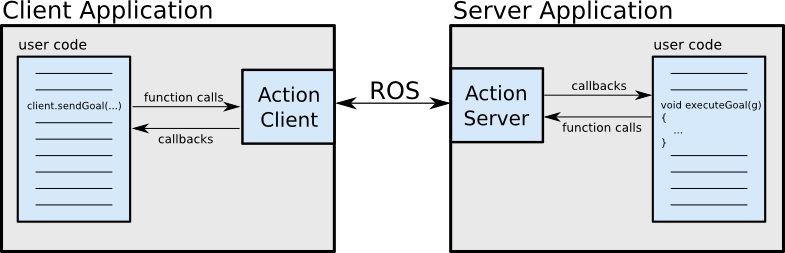
\includegraphics[width=0.8\textwidth]{client_server_interaction}
	\caption{Interaktion Client und Server}{Interaktion Client und Server\cite{actionli12:online}}
	\label{fig:clientServerInteraction}
\end{figure}

\subsection{Bags}
Bags werden in ROS gebraucht um die Daten, welche über eine Message verschickt werden zu speichern. Bags werden nicht aktiv für den Ablauf von Programmen benötigt, sind aber sehr hilfreich um Sensor- und Prozessdaten zu speichern und anschliessend auszuwerten.

\section{ROS Communityebene}
Für ROS ist, aufgrund des Open Source Aspekts, die Community ein sehr wichtiger Bestandteil des ganzen Projektes. Die ROS Community enthält ein extrem grosses Wissens- und Erfahrungspotential, dieses Wissen und die Erfahrungen wird von den einzelnen Gruppen der Community online zur Verfügung gestellt. Dazu stehen mehrere Möglichkeiten zur Verfügung:
\begin{itemize}
	\item Repositories
	\item ROS-Wiki unter \url{http://wiki.ros.org/}
	\item Bug Ticket System
	\item Mailverteiler
	\item Die 'ROS Answers'-Website	
\end{itemize} 
Das ROS-Wiki ist eine vom ROS-Konsortium erstellte Website, welche nahezu für alles ein vollständige Dokumentationen und Tutorials, mindestens aber Kurzbeschriebe, bereithält. Die ROS Answers Website bietet allen Anwendern von ROS eine Plattform in Form eines Forums um Fragen zu stellen und diese zu beantworten. Mithilfe dieser beiden Webseiten lassen sich fast alle Probleme und Unklarheiten, welche mit ROS in Verbindung stehen meistens klären.

\section{Standard Masseinheiten}
In ROS muss immer wieder mit Längen und Winkeln gearbeitet werden. Aus diesem Grund ist in ROS ein Standardisiertes Einheitensystem vorhanden. 
\begin{table}[h!]
\centering
\begin{tabular}{ll|ll}
\textbf{Grösse} & \textbf{Einheit} & \textbf{Grösse} & \textbf{Einheit} \\ \cline{1-3}
Länge           & Meter            & Leistung        & Watt             \\
Masse           & Kilogramm        & Spannung        & Volt             \\
Zeit            & Sekunden         & Temperatur      & Celsius          \\
Strom           & Ampere           & Magnetismus     & Tesla            \\
Winkel          & Radiant          & Frequenz        & Herz             \\
Kraft           & Newton           &                 &                 
\end{tabular}
\caption{Standard Masseinheiten in ROS}{Standard Masseinheiten in ROS\cite{REP103St88:online}}
\label{tab:StandardMasseinehiten}
\end{table}
\subsection{Quaternionen}
In ROS werden Rotationen nicht mit Eulerwinkeln gerechnet sondern in Quanternionen. Der grosse Vorteil von Quanternionen gegenüber der Verwendung von Eulerwinkeln ist, das bei den Quanternionen kein \gls{gimballock} entstehen kann. Quanternionen sind wie folgt definiert:
\begin{align*}
[w, x, y, z] =& [cos(\varTheta/2), sin(\varTheta/2) * nx, sin(\varTheta/2)* ny, sin(\varTheta/2) * nz]\\
\varTheta =& \text{Drehwinkel}\\
[nx,ny,nz] =& \text{Achse der Rotation}
\end{align*}

\section{Catkin}
Catkin ist das Standard Build-Tool von ROS. Catkin kombiniert CMakemakros und Pythonskripts um dem normalen CMake einige neue Funktionalitäten hinzuzufügen. Catkin wurde erstellt um das vorherige Build-Tool rosbuild abzulösen, catkin ermöglicht es Pakete mithilfe von 'find package' zu finden und mehrere voneinander abhängige Projekte gleichzeitig zu compilieren.\\
ROS nutzt ein eigenes Build-Tool um es zu ermöglichen, dass alle Pakete in ROS, unabhängig von ihrer Programmiersprache, ohne Probleme compiliert werden können. Es wird mit catkin ermöglicht voneinander abhängige Pakete zu compilieren, welche mit unterschiedlichen Programmiersprachen geschrieben wurden, andere Tools benötigen und/oder andern Organisationsstrukturen unterliegen. \cite{Allen2016}
\subsection{Workspace}
Catkin benötigt einen eigenen Workspace, welcher wie folgt initialisiert werden kann: \\
(Hier als Beispiel im Homedirectory im Ordner catkin\_ws)

\begin{code}
	\begin{minted}{bash}
	$ source /opt/ros/kinetic/setup.bash
	$ mkdir -p ~/catkin_ws/src
	$ cd ~/catkin_ws/
	$ catkin_make
	\end{minted}
	\vspace{-15pt}
	\caption{Setup eines catkin Workspace}
	\label{code:CatkinWS}
\end{code}
Anschliessend ist es zu empfehlen, dass die Variable 'ROS\_PACKAGE\_PATH' so gesetzt wird, dass der Workspace erkannt wird:

\begin{code}
	\begin{minted}{bash}
	$ echo $ROS_PACKAGE_PATH
	/home/youruser/catkin_ws/src:/opt/ros/kinetic/share
	\end{minted}
	\vspace{-15pt}
	\caption{Setzen der Umgebungsvariable}
	\label{code:PathVariable}
\end{code}

\subsection{CMakeLists}\label{Anhang:catkinCMakeLists}
Jedes Package in ROS benötigt zum compilieren durch catkin eine CMakeLists.txt Datei in ihrem Ordner. In dieser Datei werden diverse zum compilieren benötigte Einstellungen vorgenommen, unter anderem wird angegeben wo die Standard ROS-Packages zu finden sind, welche Packages zum compilieren Notwendig sind, welche der Files einen Node bilden und auch Abhängigkeiten können definiert werden. Zudem wird dem Compiler hier mitgeteilt, aus welchen Files Messages oder Services generiert werden sollen. Es ist zudem möglich und sehr zu empfehlen Flags zu setzen, welche erweiterte Fehlermeldungen bei Kompilierfehlern ausgeben. Dies vereinfacht ein Debuggen Nachfolgend sind einige der wichtigsten Zeilen aus einem CMakeFile.txt aufgeführt. Ein vollständiges CMakeFile kann im Anhang unter \ref{Anhang:Cmakelists} gefunden werden. \cite{Allen2016} \\

\begin{minipage}[H]{\textwidth}
	\begingroup
	\parfillskip=0pt
	% zwei weitere Minipages
	\begin{minipage}[t]{0.47\textwidth}        
\begin{code}
	\begin{minted}{cmake}
	find_package(catkin REQUIRED COMPONENTS
		roscpp
		geometry_msgs
		moveit_core
		moveit_ros_planning
		moveit_ros_planning_interface
		pluginlib
		cmake_modules
		message_generation
		genmsg
	)	
	\end{minted}
	\vspace{-15pt}
	\caption{Für das compilieren benötigte ROS-Packages}
	\label{code:ROSPackages}
\end{code}
	\end{minipage}%
	\hfill
	\begin{minipage}[t]{0.47\textwidth}
		\begin{code}
			\begin{minted}{cmake}
			add_executable(NodeName
				src/myROSNode.cpp
			)			
			\end{minted}
			\vspace{-15pt}
			\caption{Definieren eines Nodes aus einem .cpp-File}
			\label{code:CatkinCpp}
			
		\begin{code}
			\begin{minted}{cmake}
			add_library(LibraryName
				src/myLibrary.cpp
			)			
			target_link_libraries(targetName
				${catkin_LIBRARIES}
				LibraryName
			)			
			\end{minted}
			\vspace{-15pt}
			\caption{Hinzufügen und verlinken von Bibliotheken}
			\label{code:catkinBib}
		\end{code}
		\end{code}  
	\end{minipage}%
	\par\endgroup
\end{minipage}

\subsection{Package File} \label{sec:catkinPackageFile}
Das Package File package.xml wird von catkin gebraucht um Metadaten zu definieren. Diese beinhalten Versionsnummer, Paketname, Ersteller/Unterhalter und Lizenzen. Zudem muss angegeben werden welche anderen Packages vor dem compilieren bereits compiliert sein müssen (build\_depend), welche Packages zum compilieren benötigt werden (buildtool\_depend) und welche Packages während der Laufzeit (run\_depend) des Packages benötigt werden. Folgend ein Minimalbeispiel einer package.xml Datei. \cite{Allen2016}
\begin{code}
	\begin{minted}{xml}
<?xml version="1.0"?><package>
	<name>myPackage</name>
	<version>0.0.1</version>
	<description>My personal ROS-Package. Which does...</description>

	<maintainer email="Hans.Muster@example.com">Hans Muster</maintainer>

	<license>BSD</license>
	
	<author email="Hans.Muster@example.com">Jane Doe</author>

	<buildtool_depend>catkin</buildtool_depend>
	<build_depend>roscpp</build_depend>
	<run_depend>roscpp</run_depend>
	<build_depend>moveit_core</build_depend>
	<run_depend>moveit_core</run_depend>
	<build_depend>moveit_ros_planning_interface</build_depend>
	<run_depend>moveit_ros_planning_interface</run_depend>

	<!-- The export tag contains other, unspecified, tags -->
	<export>
	<!-- Other tools can request additional information be placed here -->
	</export>
</package>
	\end{minted}
	\vspace{-15pt}
	\caption{Minimalbeispiel einer package.xml Datei}
	\label{code:PackageXML}
\end{code}

\section{URDF}\label{sec:URDF}
Das \gls{URDF} wird gebraucht um die physikalischen Eigenschaften eines Roboters zu beschreiben. Ein URDF besteht aus einer Zusammenstellung von Links (Gliedern) und Joints (Gelenken) um eine Kinematische Kette zu bilden. (siehe Abb. \ref{fig:URDFKin})
\begin{figure} [h]
	\begin{minipage}[h]{0,49\textwidth}
		\centering
		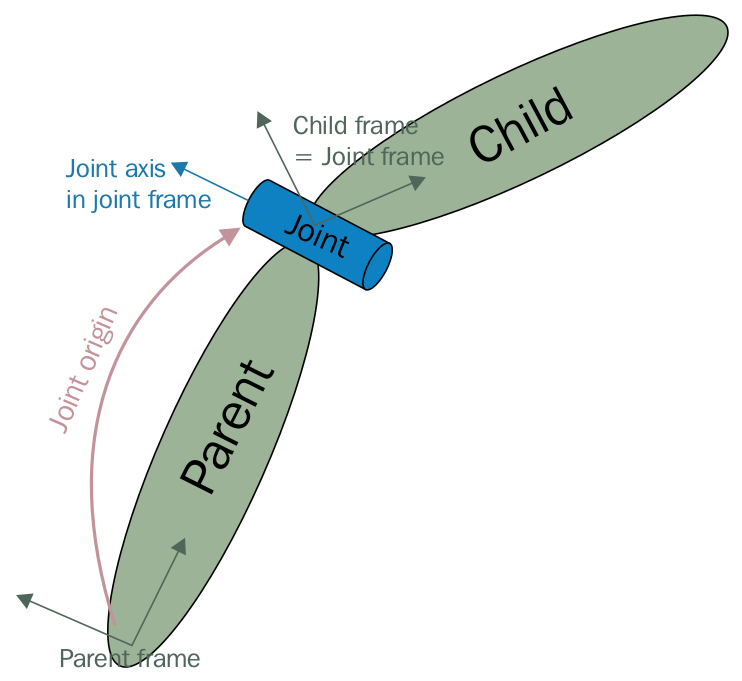
\includegraphics[width=0.95\textwidth]{URDF_kin}
		\caption[Symbolische Darstellung einer Kinematischen Kette]{Symbolische Darstellung einer Kinematischen Kette \cite{Joseph2015}}
		\label{fig:URDFKin}
	\end{minipage}
	\begin{minipage}[h]{0,49\textwidth}
		\centering
		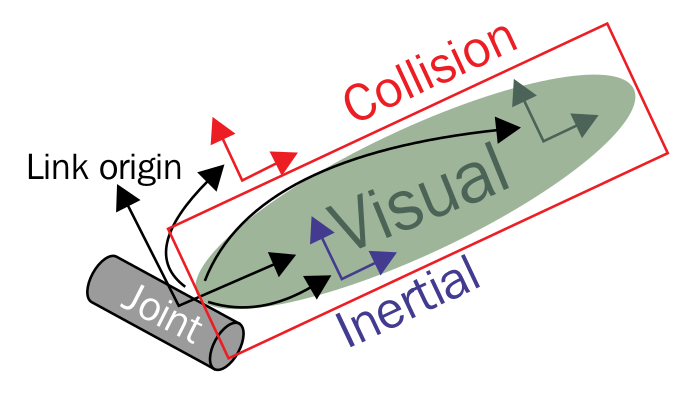
\includegraphics[width=0.95\textwidth]{URDF_link}
		\caption[Symbolische Darstellung eines Links]{Symbolische Darstellung eines Links \cite{Joseph2015}}
		\label{fig:URDFLink}
	\end{minipage}
\end{figure}

\subsection{Links}
Für jeden Link muss dabei ein Koordinatensystem und ein Geometrisches Modell definiert sein. Optional ist es möglich Massenträgheitsmomente, Farben und eine simplere Geometrie für die Kollisionsüberwachung zu definieren. Für die Geometrien ist es zudem möglich, die 3D-Objekte über importierte .stl-Files zu generieren.
\begin{code}
	\begin{minted}{xml}
<link name="base_link">
	<inertial>
		<mass value="6.215"/>
		<origin rpy="0 0 0" xyz="-0.04204 8.01E-05 0.07964"/>
		<inertia ixx="0.0247272" ixy="-8.0784E-05" ixz="0.00130902" iyy="0.0491285" iyz="-8.0419E-06" izz="0.0472376"/>
	</inertial>
	<visual>
		<origin rpy="0 0 0" xyz="0 0 0"/>
		<geometry>
			<mesh filename="package://abb_irb120_support/meshes/irb120_3_58/visual/base_link.stl"/>
		</geometry>
		<material name="">
			<color rgba="0.7372549 0.3490196 0.1607843 1"/>
		</material>
	</visual>
	<collision>
		<origin rpy="0 0 0" xyz="0 0 0"/>
		<geometry>
			<mesh filename="package://abb_irb120_support/meshes/irb120_3_58/collision/base_link.stl"/>
		</geometry>
		<material name="">
			<color rgba="1 1 0 1"/>
		</material>
	</collision>
</link>	
	\end{minted}
	\vspace{-15pt}
	\caption{Beispiel eines voll definierten Links anhand der Basis des ABB IRB120}
	\label{code:URDFLink}
\end{code}

\subsection{Joints}
Für einen Gelenk (Joint) muss definiert werden um welche Achsen sich das Gelenk drehen darf und welche beiden Links das Gelenk verbindet. Optional können Endanschläge, maximale Geschwindigkeiten, Reibungs- und Dämpfungskonstanten definiert werden. Mögliche Definitionen von Drehachsen sind revolute, continuous, prismatic, fixed, floating und planar. Nachfolgend ist ein Codeausschnitt aufgeführt, welcher ein vollständig definiertes Gelenk beschreibt.
\begin{code}
	\begin{minted}{xml}
<joint name="joint_1" type="revolute">
	<origin rpy="0 0 0" xyz="0 0 0"/>
	<parent link="base_link"/>
	<child link="link_1"/>
	<limit effort="0" lower="-2.87979" upper="2.87979" velocity="4.36332"/>
	<axis xyz="0 0 1"/>
	<dynamics damping="0.0" friction="0.0"/>
</joint>
	\end{minted}
	\vspace{-15pt}
	\caption{Beispiel eines Rotationgelenkes}
	\label{code:URDFJoint}
\end{code}

\section{MoveIt!}
MoveIt!ist eine Software zur Bewegungsplanung, Manipulation, 3D Wahrnehmung, Kinematik, Steuerung und Navigation. Es basiert auf einer Pluginstruktur, welche von ROS übernommen wurde. Dies ermöglicht es, dass MoveIt! sehr Ressourcenschonend ist und jeweils nur die Teile aktiv sind, welche auch für die jeweilige Anwendung nötig sind. Zudem ist es möglich die move\_group einfach über neue Plugins zu erweitern. Der zentrale Node in MoveIt! ist der move\_group Node, auf die Services und Actions dieses Nodes können über drei mögliche Arten zugegriffen werden:\cite{Chitta2016}

\begin{figure}[h!]
	\centering
	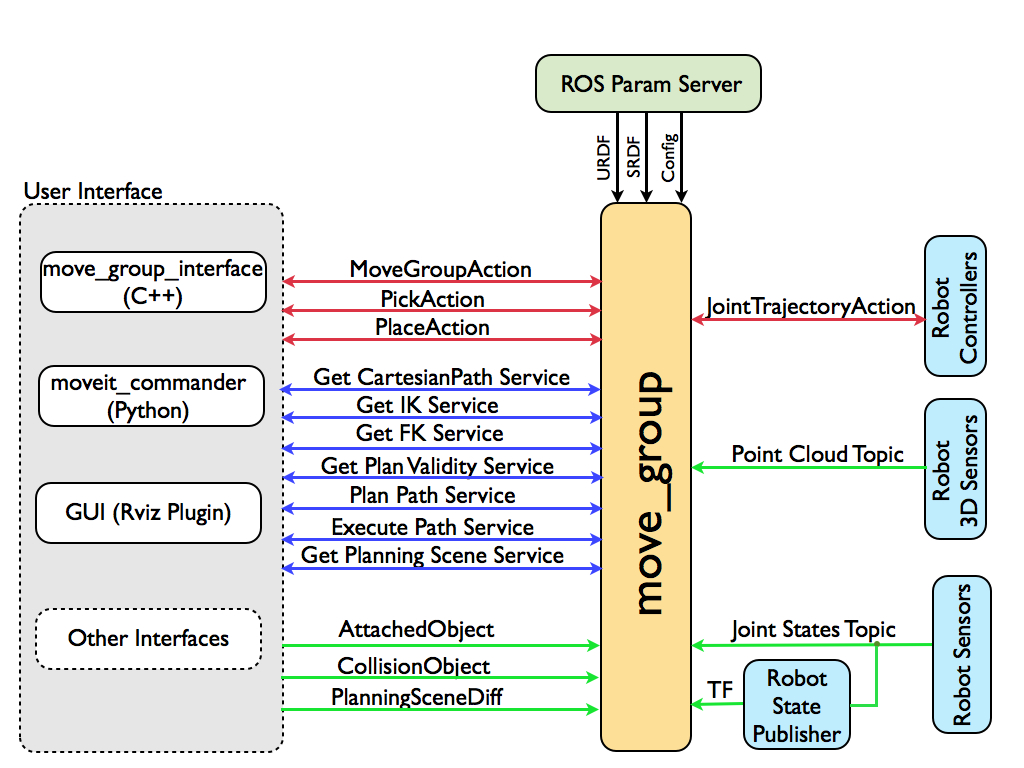
\includegraphics[width=0.8\textwidth]{move_group}
	\caption[move\_group Architektur]{move\_group Architektur\cite{Concepts23:online}}
	\label{fig:move_group}
\end{figure}

\paragraph{move\_group\_interface}
Das move\_group\_interface bietet eine API für \verb|C++|, diese eignet sich vor allem für die Erstellung komplexer Anwendungen. 
\paragraph{moveit\_commander}
Das moveit\_commander Package bietet eine API für \verb|Python|, welche sich vor allem für das erstellen von einfachen Skripts eignet. 
\paragraph{RVIZ}
Mithilfe eines Plugins für RVIZ, dem ROS eigenen Visualisierungspackage, kann die move\_group direkt über ein \gls{GUI} gesteuert werden. Dies eignet sich vor allem für schnelles Visualisieren oder das Aufsetzen eines Roboters. 

\subsection{Konfiguration}
Beim Start einer neuen move\_group bezieht diese direkt beim Parameterserver von ROS benötigte Dateien. Diese beinhalten eine URDF Datei(siehe Abschnitt \ref{sec:URDF}, welche die Physikalische Beschreibung des zu steuernden Roboters enthält. Ergänzend zum URDF wird ein SRDF benötigt, welches zusätzliche Informationen über den Roboter enthält, welche beim erstellen eines MoveIt!-Packages (siehe Abschnitt \ref{sec:ImplementierungMontage}) definiert werden. Die beiden Files (URDF und SRDF) müssen zwingend auf dem Parameterserver von ROS abgelegt sein. Zusätzlich sucht die move\_group auf dem Parameterserver noch nach weiteren, nicht zwangsweise vorhandenen, Konfigurationen. Diese können unter anderem maximale Gelenkgeschwindigkeiten, -beschleunigungen und -winkel enthalten sowie auch Daten über die Umgebung. \cite{Concepts23:online}

\subsection{Roboterinterface}
Über das Roboterinterface kommuniziert die move\_group mithilfe von ROS Topics und Actions mit dem ausgewählten Roboter.

\subsubsection{Joint State  und Transformations Informationen}
Zur Bestimmung der momentanen Position des Roboters hört die move\_group auf dem Topic /joint\_states, nach publizierten Gelenkpositionen. Diese Information geht auch über den Node Robot State Publisher welcher mithilfe eines Kinematischen Models die einzelnen Gelenkwinkel in eine genaue Position der jeweiligen Koordinatensysteme des Roboters umrechnet. Somit stehen der move\_group jederzeit die einzelnen Gelenkwinkel sowie auch die Position jeder Achse des Roboters zur Verfügung.\cite{Joseph2015}

\subsubsection{Controller Interface}
Die move\_group sendet Bewegungsbefehle über das FollowJointTrajectoryAction Interface, welches von ROS zur Verfügung gestellt wird, auf den entsprechenden Roboter Controller. Dabei ist zu beachten, dass auf dem Controller vorgängig ein entsprechender Actionserver implementiert werden muss, welcher die Anfragen in Steuerungsbefehle umwandelt. \cite{Joseph2015}

\subsection{MoveIt! Setup Assistant}
Der MoveIt! Setup Assistant ist ein sehr hilfreiches Tool welches ermöglicht jegliche Art von Roboter zu Konfigurieren so, dass dieser anschliessend mit MoveIt! respektive der move\_group gebraucht werden kann. Dazu benötigt der Setup Assistant ein gültiges URDF-File, aus welchem ein SRDF-File und andere für MoveIt! und die Bewegungsplanung benötigten Files generiert werden. Dank dem \gls{GUI} des Setup Assistants wird einem das erstellen des configuration packages sehr erleichtert. Dazu müssen folgende Schritte abgearbeitet werden:\cite{Industri70:online}
\begin{enumerate}
	\itemsep0pt
	\item Starten und URDF laden
	\item Generieren der Selbstkollisionsmatrix
	\item Virtuelle Gelenke hinzufügen
	\item Planungsgruppen erstellen
	\item Roboterposen hinzufügen
	\item Endeffektoren hinzufügen
	\item Passive Gelenke hinzufügen
	\item Konfigurationsfiles generieren	
\end{enumerate}
Der Setup Assistant kann über ein Linux Terminal mit folgendem Befehl gestartet werden:\\
\mintinline{bash}{$ roslaunch moveit_setup_assistant setup_assistant.launch}\\ %$
Eine ausführlichere Beschreibung anhand eines Beispiels ist im Abschnitt \ref{sec:MoveitSetup} aufgeführt.

\subsection{Planningscene}
Die Planningscene beinhaltet eine Repräsentation der echten Welt, in ihr ist der Roboter in seinem momentanen Zustand abgebildet, sowie auch alle Objekte welche sich momentan im Arbeitsraum des Roboters befinden. Die Planningscene wird für die Bestimmung von Kollisionsberechnungen gebraucht. \cite{Pan2012}

\subsection{Kollisionsüberwachung}
Auch für die Kollisionsüberwachung wird eine Bibliothek über ein Plugin implementiert, standardmässig ist dies die \gls{FCL}. Dabei werden die folgenden Geometrischen Formate unterstützt:\cite{Pan2012}
\begin{itemize}
	\itemsep0pt
	\item Meshes: .stl oder .dae
	\item Primitive Shapes: Boxen, Zylinder, Kugeln, etc.
	\item \gls{octomap}: kann direkt für Kollisionsüberwachung gebraucht werden
\end{itemize}
Beim erstellen eines neuen MoveIt! Packages kann mithilfe des MoveIt! Setup Assistants eine Kollisionsmatrix erstellt werden, welche definiert welche Körper für die Berechnung der Kollision vernachlässigt werden können weil sie zum Beispiel gar nicht kollidieren können. Dies erspart einen grossen Teil an Rechenleistung und somit können Bahnplanungen schneller durchgeführt werden.\cite{Chitta2016}

\subsection{Kinematischer Solver}
Zur Lösung von Kinematikberechnungen sind in MoveIt! standardmässig zwei numerische kinematische Solver über ein Plugin implementiert.\cite{Chitta2016} Bei diesen Solvern handelt es sich um KDL und LMA beide basieren auf der \gls{KDL} von Orocos.\cite{Kinemati93:online} Zusätzlich wurde der Planer Trac-IK von Traclabs installiert, welcher laut den Angaben von Traclabs massiv schneller und zuverlässiger Lösungen finden soll, als die beiden Standardsolver.\cite{traclabs28:online} Es muss je nach Roboter ausgetestet werden, welcher Solver bessere Ergebnisse liefert.

\subsection{Bewegungsplanung}
MoveIt! implementiert Bewegungsplaner über ein Plugin, dies ermöglicht es einfach zwischen mehreren Bewegungsplanungsbibliotheken zu wechseln, gleichzeitig ist es möglich einen eigenen Anwendungsspezifischen Bewegungsplaner in MoveIt! zu implementieren. Die Standard mässig implementierte Planungsbibliothek ist \gls{OMPL}. Mithilfe des MoveIt! Setup Assistant können die einzelnen Planer Konfiguriert werden.\cite{Chitta2016} \\

Um ein Grundverständnis für die Planer zu entwickeln wird in diesem Abschnitt kurz auf die in OMPL verfügbaren Planer eingegangen, aufgrund der Komplexität der Planer wird auf eine ausführlichere Beschreibung verzichtet. 
Grundsätzlich können die Planer welche in \gls{OMPL} vorhanden sind in zwei Kategorien unterteilt werden. Es gibt geometrische Planer und Kontrollbasierte Planer.\cite{Availabl94:online}
\subsubsection{Geometrische Planer}
Geometrische Planer berücksichtigen bei der Bahnplanung nur geometrische und kinematische Beschränkungen. Dabei trifft der Planer die Annahme, dass jeder vom Bahnplaner gefundene Weg in eine Bahn umgewandelt werden kann welche Dynamisch auch fahrbar ist. Dabei können diese Planer wieder  in folgende Unterkategorien unterteilt werden:\cite{Availabl94:online}
\paragraph{Single-query Planer} Diese Planer bauen eine Baumstruktur auf, welche aus gültigen Bewegungen besteht und sich vom Start in Richtung Ziel bewegen. Einige Planer bauen die Baumstruktur gleichzeitig von Ziel und Start auf und treffen sich in der Mitte. Die einzelnen Planer dieses Typs unterscheiden sich hauptsächlich darin, wann und wo die Baumstruktur erweitert wird.\cite{Availabl94:online}
\paragraph{Multi-query Planer} Diese Art von Planern erstellt vorgängig eine Karte der ganzen Umgebung, welche anschliessend genutzt wird um zu bestimmen ob sich die berechneten Bewegungen innerhalb dieser Karte befinden und somit gültig sind.\cite{Availabl94:online}
\paragraph{Optimierende Planer} Optimierende Planer wählen gefundene Wege aufgrund von Optimierungskriterien, normalerweise ist dies die Distanz welche kurz gehalten werden soll. Es ist jedoch auch möglich, zum Beispiel die mechanische Arbeit zu minimieren. Obwohl das finden eines optimalen Weges von Vorteil ist, ist zu beachten, dass optimierende Planer die ihnen zur Verfügung gestellte Rechenzeit in der Regel komplett ausnutzen. Somit sind die gefahrenen Wege meistens kürzer als bei den Queryplanern es ist aber möglich, dass die gesparte Fahrzeit in längerer Rechenzeit verloren geht.\cite{Lav06}

\subsubsection{Kontrollbasierte Planer}
Kontrollbasierte Planer setzen nicht nur auf geometrische und kinematische Beschränkungen. Es werden Zustandsdarstellungen benutzt, um einzelne Positionen auf dem Weg zu definieren. Über Algorithmen wird bewertet wie hoch der Steuerungsaufwand ist um von Zustand zu Zustand zu gelangen, dieser soll möglichst klein gehalten werden. \cite{Availabl94:online}

\subsection{Trajektorienberechnung}
Die aus der Bewegungsplanung berechneten Bahnen beinhalten noch keine Zeitinformationen, aus diesem Grund ist in MoveIt! ein Plugin zur Trajektorienberechnung implementiert. Dieses Plugin berechnet aufgrund der in den Konfigurationsdateien abgespeicherten erlaubten Gelenkgeschwindigkeiten aus der berechneten Bahn eine Trajektorie. Auch hier ist es wieder möglich, über ein Plugin eine eigene Version der Trajektorienberechnung zu implementieren. \cite{Chitta2016}

\section{ROS Industrial}
ROS-Industrial erweitert das von ROS zur Verfügung gestellte Framework rund um Industrierobotik und -automation. Die Erweiterung durch ROS-Industrial umfasst eine Vielzahl von Interfaces für diverse in der Industrie gebräuchliche Hardware, wie zum Beispiel Greifer oder Sensoren. Zudem sind in dem ROS-Industrial Repository\footnote{https://github.com/ros-industrial/} diverse Bibliotheken verfügbar, welche die spezifisch auf die Anwendung im Rahmen der Industrie zugeschnitten sind. ROS-I wird durch ein Konsortium\cite{ROS-IMembers} an Forschergruppen sowie auch von Firmen aus der Industrie unterstützt.
Folgend sind einige Vorteile und Eigenschaften, der ROS-I Beschreibung aufgeführt:\cite{Descript37:online}
\begin{itemize}
	\itemsep0pt
	\item Implementiert die bereits mächtigen Funktionen aus ROS
	\item Ermöglicht neue Applikationen
	\item Vereinfacht die Roboterprogrammierung bis auf die Taskebene
	\item Reduziert Kosten
	\item Open Source
\end{itemize}
ROS-Industrial kann grundsätzlich in zwei Pakettypen unterteilt werden. Zum einen gibt es die ROS-I spezifischen Pakete, diese beinhalten alle generell in ROS-I brauchbaren Funktionen. Zum anderen gibt es die herstellerspezifischen Pakete, diese beinhalten die benötigten Beschreibungs- sowie Setupfiles, um einen Roboter eines bestimmten Herstellers in Betrieb zu nehmen. 
\subsection{Unterstützte Hersteller}
ROS-I arbeitet eng mit diversen Forschungseinrichtungen sowie auch Herstellern zusammen und unterstützt bereits von Haus aus diverse Hardware von einigen Herstellern. Gleichzeitig gibt es eine sehr grosse Anzahl an Paketen und Bibliotheken, welche durch die Open Source Community erstellt wurden aber nicht offiziell - oder zumindest noch nicht - von ROS-I unterstützt werden.
\begin{table}[H]
	\centering
	\begin{tabular}{llll}
		\textbf{Hersteller} & \textbf{Controller(s)} & \textbf{Manipulator} & \textbf{MoveItPkg} \\ \hline
		ABB                 & IRC5                   & IRB-2400             & YES                \\
		                    &                        & IRB-5400             & NO                 \\ \hline
		Adept               & CX, CS                 & Viper 650            & NO                 \\ \hline
		Fanuc               & R-30iA / R-30iB        & LR Mate 200iC (all)  & YES                \\
		                    &                        & LR Mate 200iD        & YES                \\
		                    &                        & M-10iA               & YES                \\
		                    &                        & M-16iB/20            & YES                \\
		                    &                        & M-20iA(/10L)         & YES                \\
		                    &                        & M-430iA/(2F, 2P)     & YES                \\
		                    &                        & M-900iA/260L 5       & NO                 \\ \hline
		Motoman             & DX100                  & SIA10D/F             & NO                 \\
		                    &                        & FS100                & NO                 \\
		                    &                        & DX200                & NO                 \\
		                    &                        & YRC1000              & NO                 \\ \hline
		Universal Robot     & CB2/CB3 10             & UR 5                 & YES                \\
		                    &                        & UR 10                & YES                \\ \hline
	\end{tabular}
	\caption[Offiziell unterstützte Hardware]{Offiziell unterstützte Hardware\cite{HardwareSup:online}}
	\label{tab:hersteller}
\end{table}

\subsection{Robot Support Package}
Robotsupportpackages werden von ROS-Industrial verwendet um alle Dateien an einem Ort zu sammeln, welche nötig sind um einen Industrieroboter zu betreiben, respektive eine MoveIt! Konfiguration dafür zu erstellen. Die Strukturen, Namensgebungen sowie auch Funktionen in einem ROS-I Package unterliegen in diverser Konvention. 
\subsubsection{Ordnerstruktur}
Übersichtshalber ist der Inhalt solcher Packages definiert, es wird auch empfohlen beim erstellen solcher Packages sich an die Ordnerstruktur sowie an die Namenskonventionen zu halten. Die Ordnerstruktur sieht in folgendermassen aus:\\
\dirtree{%
	.1 RoboterName\_support.
	.2 config.
	.2 launch.
	.2 meshes.
	.2 test.
	.2 urdf.
}
\subsubsection{Launchfiles}
Durch ROS-Industrial werden einige .launch-Files vorgegeben, welche in jedem Support Package vorhanden sein müssen. Diese werden teils automatisch generiert, andere müssen selber geschrieben werden. Nachfolgend eine Auflistung der .launch-Files und eine kurze Beschreibung ihrer Funktion.
\begin{description}
	\item[load\_roboterName.launch] Lädt alle roboterspezifischen Konfigurationsdateien, welche von MoveIt! benötigt werden auf den ROS Parameterserver.
	\item[test\_roboterName.launch] Startet RVIZ und ermöglicht es die Konfiguration der Gelenke zu überprüfen. Dafür werden die beiden Nodes joint\_state\_publisher und robot\_state\_publisher gestartet.
	\item[robot\_state\_visualize\_roboterName.launch] Visualisiert den Zustand eines echten oder simulierten Roboters in RVIZ. Es können dem Robotercontroller dabei keine Befehle erteilt werden.
\end{description}
Das letzte .launch-File ist das robot\_interface welches eine bidirektionale Kommunikation mit dem Robotercontroller startet. Dieses .launch-File gibt es in zwei unterschiedliche Versionen, abhängig vom Controller. Diese unterscheiden sich darin, wie ROS-I mit dem Robotercontroller kommuniziert. 
\begin{description}
	\item[robot\_interface\_download\_roboterName.launch] Das Download Interface sendet die gesamte berechnete Trajektorie in einem Paket an den Controller, dieser führt diese Anschliessend aus. Beim Erhalt eines neuen Trajektorienpakets wird der Roboter gestoppt und die alte Trajektorie verworfen. 
	\item[robot\_interface\_streaming\_roboterName.launch] Beim Streaming Interface werden die generierten Trajektorienpunkte direkt an den Controller gesendet, welcher leicht Zeitverzögert die ankommenden Trajektorienpunkte ausführt.
\end{description}

\subsection{Standardisierte Links}
Gemäss ROS-I sind drei Links definiert, welche in jedem Package gleich benennt sein müssen. Einerseits der base\_link welcher die Basis des Roboters bildet, an welcher dieser befestigt wird. Der tool0 Link ist der letzte Link eines Roboters, er befindet sich somit im Zentrum des \gls{TCP}, seine Orientierung entspricht der Orientierung des Standard Toolframes des Roboters. Der dritte definierte Link ist der flange\_frame, gemäss der Definition von ROS-I entspricht seine Position dem Befestigungspunkt des jeweiligen Endeffektors. Die Orientierung ist genormt mit der x-Achse in Vorwärtsrichtung, y nach links und z nach oben.

\subsection{URDF's und xacro}
Die physikalischen Beschreibungen eines industriellen Roboters werden nicht in einem URDF verfasst, sondern in einem .xacro-File. Diese sind vom Syntax her identisch, jedoch erlauben es .xacro-Files Macros zu verwenden. Mithilfe von Macros können Tags generiert werden, welche es ermöglichen andere .xacro-Files zu suchen und Importieren. Zudem ist es möglich jedem Gelenk und Glied eines Roboters ein Präfix zu geben. Dies verhindert bei mehrfacher Verwendung eines .xacro-Files Namenskonflikte, falls ein xacro mehrfach verwendet werden will.
Aus einem .xacro-File muss kann anschliessend wieder ein URDF generiert werden. 
%!TEX root = ../doc.tex
\chapter{ROS: Setup und Tools}\label{sec:rosSetup}
Damit mit ROS und ROS-I gearbeitet werden kann müssen zuerst einige Installationen und Setups vorgenommen werden. Diese werden in diesem Abschnitt erläutert. Gleichzeitig werden einige ROS spezifische Tools erläutert, die das Arbeiten und auch Debuggen erleichtern können.
\section{Auswahl Distribution}
Für die Implementierung des Basis ROS-Systems, sowie für ROS-Industrial musste eine geeignete ROS-Distribution (siehe Abschnitt \ref{sec:Distro}) gewählt werden. Die Wahl viel Dabei auf die Distribution ROS Kinetic Kame. Diese Distribution wurde gewählt, da sie im Vergleich zu ihrer Vorgängerversion (ROS Jade Turtle) einige Verbesserungen mit sich bringt. Gleichzeitig ist es von Vorteil, dass die Distribution schon ca. ein Jahr im Einsatz ist und somit ein Grossteil der verfügbaren Packages von ROS schon auf die Version Kinetic porträtiert wurden.

\section{Auswahl IDE}
Grundsätzlich kann Sourcecode in ROS, wie jede andere Software auch, mit einem Texteditor und einem passenden Compiler generiert werden. Für ROS stehen eine Vielzahl an \glspl{IDE} zur Verfügung. Aufgrund von bereits vorhandener Erfahrung wurde Visual Studio Code verwendet, welches mit einem Plugin erweitert werden kann um CMakeFiles und auch ROS spezifische Files besser zu unterstützen. 

\section{Installation}
Die Installation von ROS und ROS-I können in Ubuntu über \gls{apt} installiert werden. Eine detaillierte Installationsanleitung ist auf dem ROS-Wiki\footnote{ROS: \url{http://wiki.ros.org/kinetic/Installation}\\ROS-I:\url{http://wiki.ros.org/Industrial/Install}} zu finden. Hier wird nur auf die wichtigsten Details eingegangen, da die Installationsanleitung eher umfangreich ist. Wichtig bei der Installation ist, das für ROS und ROS-Industrial die selben Distributionen installiert werden, zudem ist es zu empfehlen alle ROS und ROS-I Packages zu installieren. Dies verhindert spätere Komplikationen durch nicht vorhandene Packages. Nach der Installation von ROS sollten direkt die Abhängigkeiten von ROS initialisiert (\mintinline{bash}{rosdep init}) und upgedatet (\mintinline{bash}{rosdep update}) werden.\\
\newpage
\section{Workspace}
Nach der Installation muss ein Workspace eingerichtet werden welcher für Catkin konform ist. Dies über die \gls{IDE} möglich, geht aber am einfachsten über folgende Konsolenbefehle:
\begin{code}
	\begin{minted}{bash}
$ source /opt/ros/kinetic/setup.bash	# Source ROS setupscript
$ mkdir -p ~/catkin_ws/src				# erstellen benötigter Ordner	
$ cd ~/catkin_ws/
$ catkin_make							# compilieren
$ source devel/setup.bash				# Source Workspace setupscript
	\end{minted}
	\vspace{-15pt}
	\caption{Konsolenbefehle zur Generierung eines Catkin-Workspace}
	\label{code:catkinWS}
\end{code}
Im Workspace sollten sich nun die Unterordner build und devel befinden, gleichzeitig sollte sich im Ordner src die Datei CMakelists.txt befinden.
Das Setupscript eines Workspaces muss beim starten eines neuen Terminals immer neu eingelesen werden, es bietet sich an diese Zeile im File \verb|~/.basrc| hinzuzufügen, damit dies nicht mehr notwendig ist. 

\section{Nützlichetools}
In ROS gibt es eine Vielzahl nützlicher Konsolenbefehle und Tools hier eine kurze Auflistung der in dieser Arbeit meist gebrauchten.

\subsection{rqt}
Bei rqt handelt es sich um ein sehr mächtiges Tool in ROS, welches es ermöglicht auf fast alle Datenströme (messages, topics, services) zuzugreifen und diese zu visualisieren. Das Standartmenü kann über die Konsole mit dem Befehl \mintinline{bash}{rqt} gestartet werden, dazu muss jedoch bereits ein ROS-Master aktiv sein. Mithilfe diverser Plugins können weitere nützliche Funktionen von rqt genutzt werden. Eine der Hilfreichsten ist dabei rqt\_graph welche mit dem gleichlautenden Konsolenbefehl gestartet werden kann. Mit rqt\_graph können alle aktiven Nodes und die auf den Topics publizierten Nachrichten visualisiert werden. Somit kann schnell und einfach überprüft werden, ob ein Node läuft und ob Topics vorhanden sind. 
\begin{figure}[h!]
	\centering
	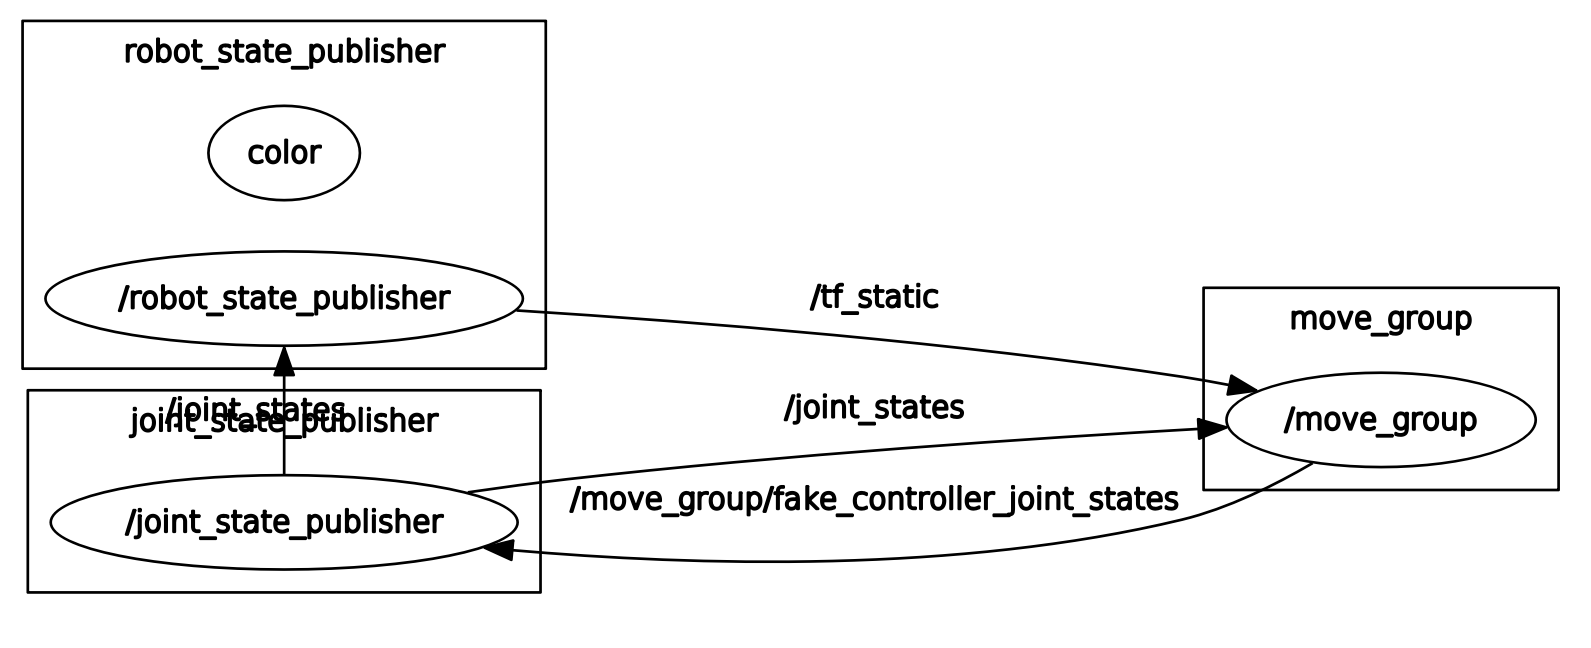
\includegraphics[width=0.8\textwidth]{rqtGraph}
	\caption{Ausgabe von rqt\_graph}
	\label{fig:rqtGraph}
\end{figure}

\subsection{Node}
\begin{description}[align=left]
	\item[rosnode list] Gibt eine Liste aller laufenden Nodes aus
	\item[rosnode info nodename] Gibt Informationen über einen laufenden Node aus
	\item[rosnode ping nodename] Pingt einen laufenden Node
	\item[rosnode kill nodename] Beendet einen laufenden Node
\end{description}

\subsection{Topics}
\begin{description}[align=left]
	\item[rostopic list] Gibt eine Liste mit allen registrierten Topics aus
	\item[rostopic echo /topicname] Gibt alle auf dem Topic publizierten Nachrichten aus
	\item[rostopic hz /topicname] Gibt die Frequenz an mit der Publiziert wird
	\item[rostopic pub /topicname data] Publiziert auf einem Topic die mitgegebenen Daten
\end{description}

\subsection{Parameterserver}
\begin{description}
	\item[rosparam list] Gibt eine Liste aller gespeicherten Parameternamen aus
	\item[rosparam get /paramname] Gibt den gespeicherten Variabelwert zurück
	\item[rosparam set /paramname] Über-/schreibt einen neuen Wert auf den Parameterserver
	\item[rosparam delete /paramname] Löscht den angegebenen Parameter vom Server
\end{description}


%!TEX root = ../doc.tex
\chapter{Industrie Demonstrator}
\label{sec:montageaufgabe}
In der Bachelorarbeit von Andrin Meister und Christian Hartmann wurde ein Grossteil des Aufbaus und der Funktionalitäten des Industrie 4.0 Demonstrators definiert. In den folgenden Abschnitten wird kurz auf die für den Montageprozess mit dem Sechsachsroboter der Firma Stäubli wichtigsten Punkte eingegangen. 

\section{Physikalische Schnittstellen}\label{sec:HWSchnittstellen}
Der Industrie Demonstrator ist modular Aufgebaut, es gibt 3 trennbare Module, die Montagezelle mit dem Industrieroboter befindet sich in der mittleren Zelle. Der Arbeitsraum des Roboters ist nahezu nicht durch andere Systeme im Demonstrator beschränkt. Die einzigen physikalischen Interaktionen mit dem gesamt System bestehen aus dem Greifen der Teile aus den Teileträgern, welche auf Linearschlitten montiert sind. Auch im Mittelteil der Anlage wird ein Portalroboter verbaut, welcher sich in der Nähe des Sechsachsroboters bewegt. 
\begin{figure}[h!]
	\centering
	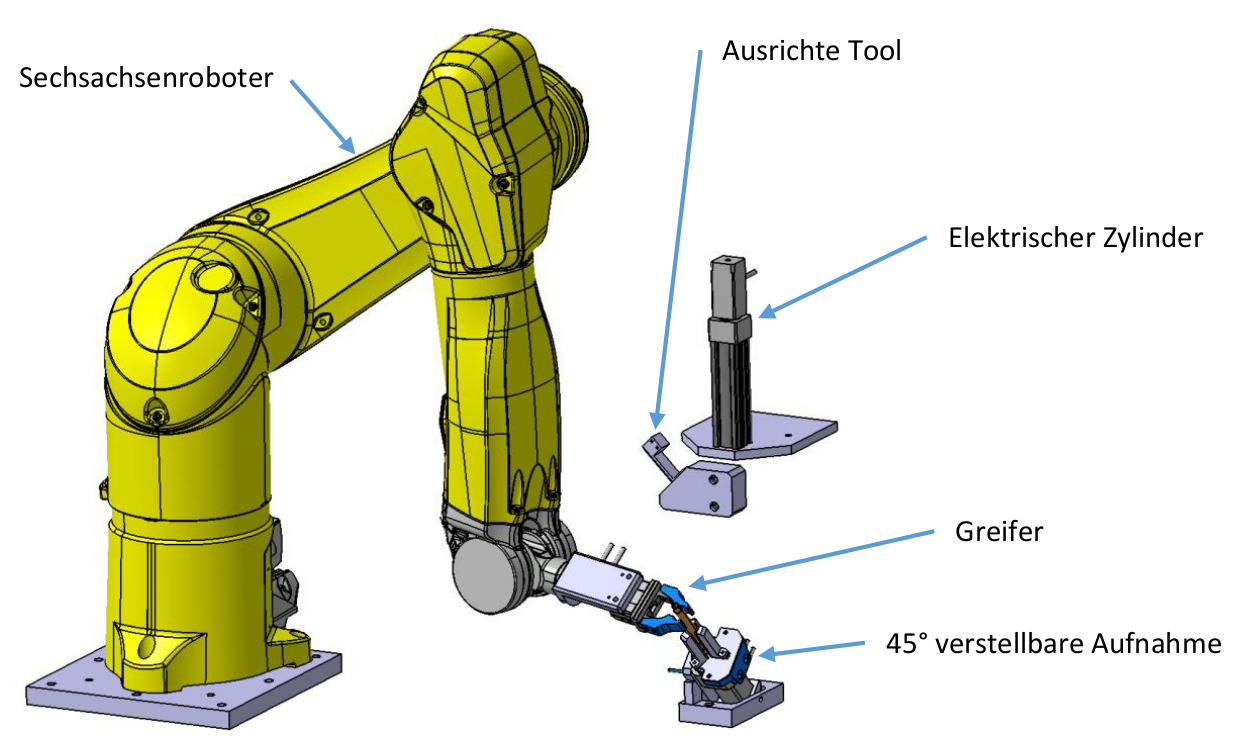
\includegraphics[width=0.8\textwidth]{workcell}
	\caption[Hauptelemente der Montagestation]{Hauptelemente der Montagestation\cite{Hartmann2017}}
	\label{fig:workcell}
\end{figure}

\section{Software Schnittstellen}\label{sec:SWschnittstellen}
Der Grossteil der Anlage wird über Siemens SPS Steuerungen angesteuert, welche über PROFINET kommunizieren. Eine Einbindung dieses Protokolls in eine Linux/ROS Umgebung ist sehr komplex. Aus diesem Grund wurde mit den restlichen am Industrie 4.0 Demonstrator beteiligten Personen definiert, dass der der Linux PC gegen Aussen ein Webserver zur Verfügung stellt. Der zentralen Steuerung der Anlage soll es dabei möglich sein, einen Montagevorgang auszulösen sowie den Status des Roboters abzufragen. \\
Von ROS aus muss zudem die Ansteuerung des Dreibackengreifers, der Presse, sowie des Greifers am Roboterarm geschehen. Bei all diesen Aktuatoren handelt es sich um Servomotoren der Firma SMC welche mit Controllern mit einem EtherCAT Interface angesteuert werden können.

\section{Kugelschreibermontage}
Der Kugelschreiber, welcher zusammengebaut werden soll, besteht aus insgesamt aus fünf Teilen. Diese Einzelteile liegen definiert im Schlitten des Transportsystems, welche an einer vordefinierten Stelle im Arbeitsbereich des Roboters anhalten. Diese Teileträger befinden sich während des ganzen Montageprozesses an der selben Position.
Der Montageablauf besteht aus folgenden Schritten:
\begin{enumerate}
	\item Vorderhülle in Dreibackengreifer positionieren
	\item Vorderhülle mithilfe des ausrichte Tools in korrekte Position drehen
	\item Feder in Vorderhülle einführen
	\item Miene in Vorderhülle einführen
	\item Arretierung aufsetzen
	\item Dreibackengreifer inkl. Kugelschreiber in senkrechte Lage drehen
	\item Deckel positionieren und aufpressen
	\item Dreibackengreifer inkl. Kugelschreiber in 45\textdegree Lage drehen
	\item Kugelschreiber entnehmen
\end{enumerate}
Der Grundsätzliche Ablauf für die Montage des Kugelschreibers ist durch die Geometrie des Kugelschreibers gegeben, wie genau diese Teile gegriffen werden und wie die Montagestation aufgebaut ist wurde in der Bachelorarbeit von Andrin Meister und Christian Hartmann definiert und sind somit für diese Arbeit vorgegeben. Für genauere Details zur Auswahl und Definition ist die Bachelorarbeit hinzuzuziehen.
%!TEX root = ../doc.tex
\chapter{Implementierung MoveIt! Package}\label{sec:ImplementierungMontage}
Im folgenden Kapitel wird anhand des Stäubli Roboters TX2-60l erläutert, wie das MoveIt! Package für ROS-I erzeugt wird. Dieses Vorgehen wurde mit leichten Abänderungen auch auf den IRB120 von ABB und den UR3 von Universal Robots angewendet. Es ist wäre auch möglich andere Roboter so in den Industrie Demonstrator einzubinden.\\

Zur Erzeugung des MoveIt! Packages wird ein .xacro File benötigt. Für den IRB120 und UR3 sind diese Pakete bereits im ROS-I Gitrepository vorhanden, wobei das Package für den IRB120 unter dem Status experimentell aufgeführt wird. Die für den Stäubliroboter generierten Files werden im Ordner /staubli\_expermiental/staubli\_tx260l\_support abgelegt. Für den Stäubli Roboter musste ein Package aufgesetzt werden. Dazu wurden folgende Schritte durchgeführt:
\begin{enumerate}
	\item Erstellen Visual- und Kollisionsmodelle
	\item Erstellen .xacro File
	\item Generieren MoveIt! Package
	\item Anpassungen für ROS-I
\end{enumerate}

\section{Erstellen Visual- und Kollisionsmodelle}
\subsection{Roboter und Greifer}
Die CAD-Modelle des TX2-60l wurden von der Website von Stäubli bezogen, anschliessend musste an den Modellen gemäss den ROS/ROS-I Konventionen einige Anpassungen gemacht werden. Diese beinhalten vor allem Anpassungen am Koordinatensystem. Die ROS-Konventionen bestimmen, dass relativ zu den Körpern die x-Achse nach vorne Zeigt, die y-Achse nach links und die z-Achse nach oben.\\
Damit an Rechenleistung gespart werden kann, werden für die Kollisionsberechnung vereinfachte CAD-Modelle verwendet. Diese wurden mithilfe der Software Meshlab, welche gratis verfügbar ist, erstellt. Meshlab bietet diverse Tools und Funktionen um .stl-Files, sowie auch andere Tesselationsfiles zu bearbeiten. Für die Kollisionsfiles werden die CAD-Files mithilfe des Tools 'Convex Hull' vereinfacht (Vergleich Abbildung \ref{fig:Collision} und \ref{fig:visual}). Die erstellten Modelle werden in den entsprechenden Unterordnern abgelegt.\\

\begin{figure} []
	\begin{minipage}[h]{0,49\textwidth}
		\centering
			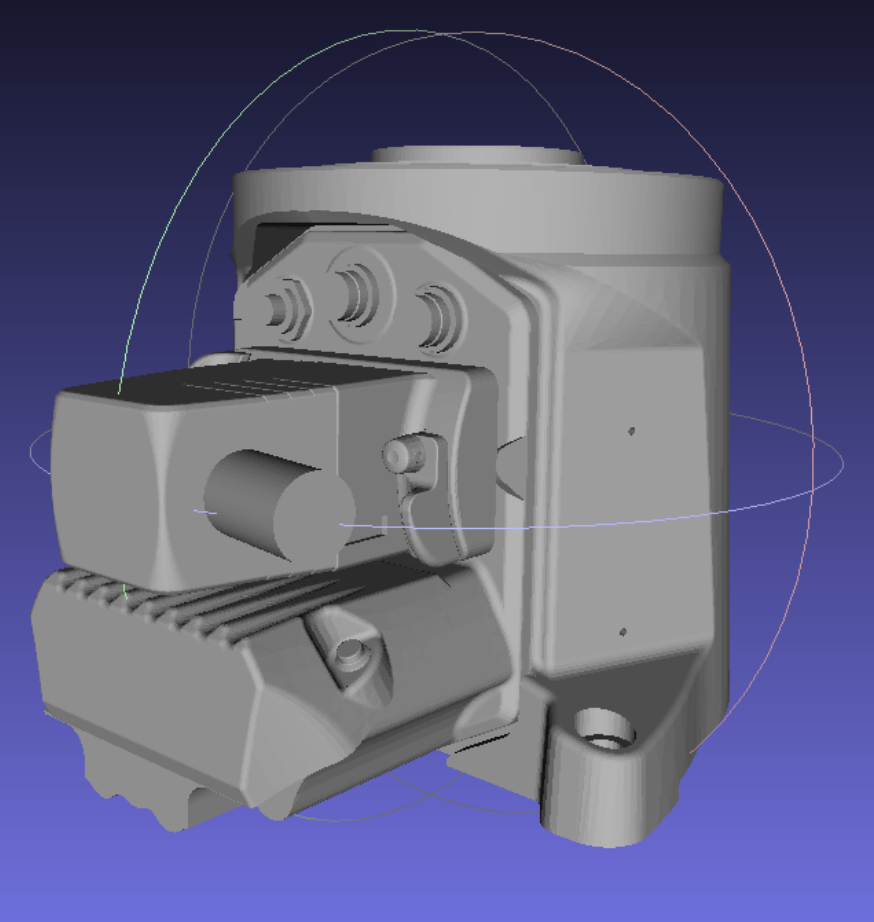
\includegraphics[width=0.95\textwidth]{visual}
		\caption{Visuelles Modell der Base TX2-60l}
		\label{fig:visual}
	\end{minipage}
	\begin{minipage}[h]{0,49\textwidth}
		\centering
			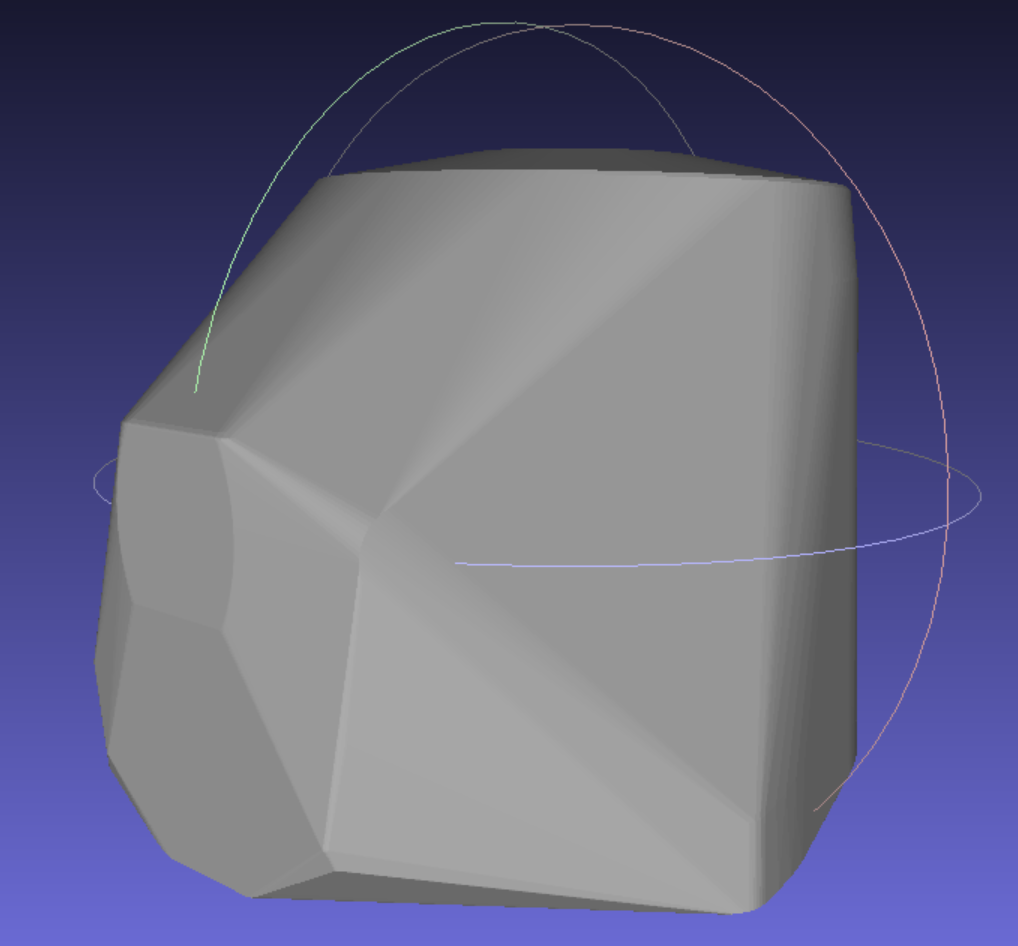
\includegraphics[width=0.95\textwidth]{collision}
		\caption{Kollisions Modell der Base TX2-60l}
		\label{fig:Collision}
	\end{minipage}
\end{figure}
Das selbe Vorgehen wurde auch für den Greifer durchgeführt, bei diesem wurde die Convex Hull jedoch nur auf den hinteren Teil des Greifers angewendet.  

\subsection{Anlage}
Aufgrund der Grösse und Komplexität der Anlage ist auch das CAD-Modell sehr gross. MoveIt! hat starke Schwierigkeiten sehr grosse Files zu laden, aus diesem  Grund wurde der visuelle Teil der Anlage mithilfe von Meshlab stark vereinfacht. Somit konnte die Dateigrösse von 240MB auf circa 50MB verringert werden, diese Grösse lässt sich einigermassen gut importieren und visualisieren.\\
Für das Kollisionsmodell wurde nur der mittlere Teil der Anlage verwendet und stark vereinfacht. Ein Grossteil wird dabei einfach als Box dargestellt (siehe Abbildung \ref{fig:collisionAnlage}).

\begin{figure} [H]
	\begin{minipage}[h]{0,49\textwidth}
		\centering
		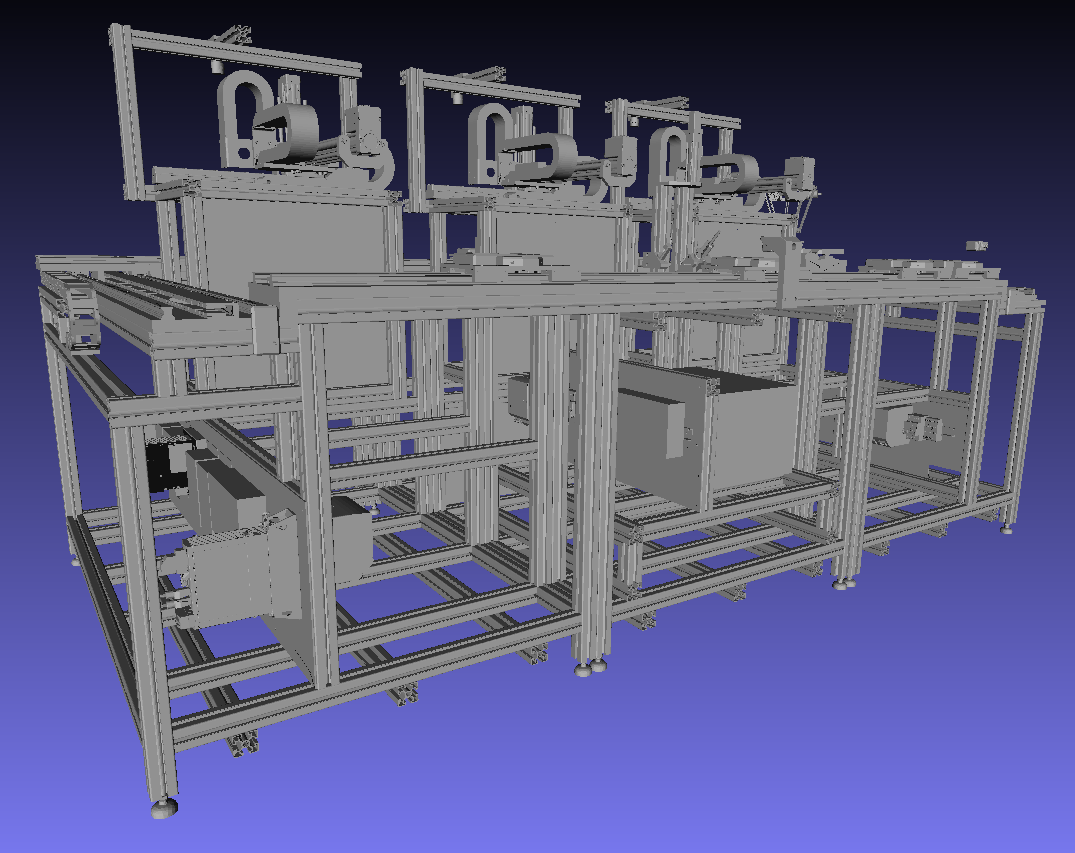
\includegraphics[width=0.95\textwidth]{visualAnlage}
		\caption{Visuelles Modell}
		\label{fig:visualAnlage}
	\end{minipage}
	\begin{minipage}[h]{0,49\textwidth}
		\centering
		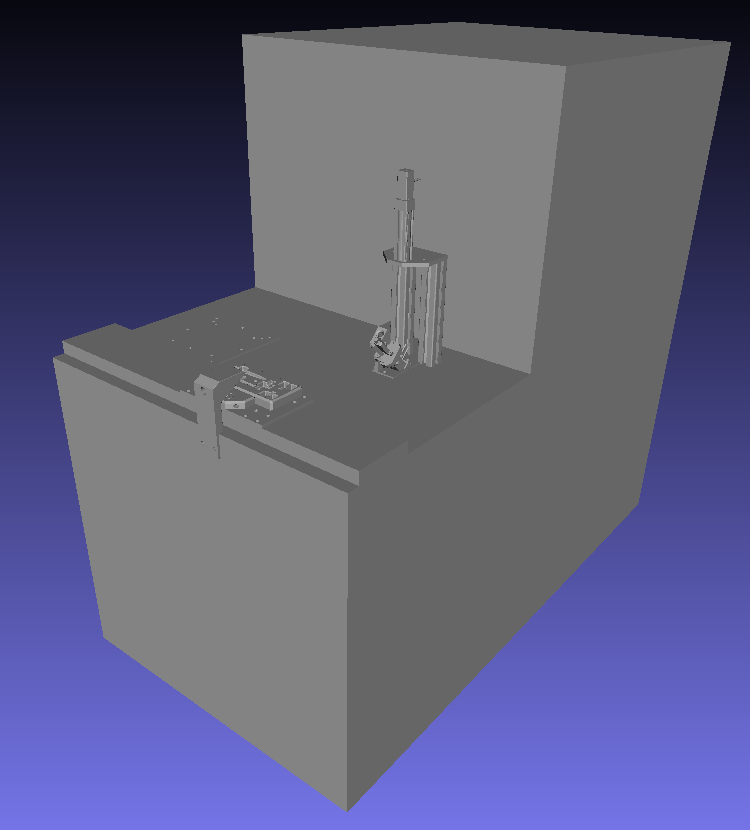
\includegraphics[width=0.95\textwidth]{collisionAnlage}
		\caption{Kollisions Modell}
		\label{fig:collisionAnlage}
	\end{minipage}
\end{figure}

\section{xacro Files}
Für die Einbindung des Roboters in die Montageanlage wurden vier unterschiedliche xacro-Files erstellt. Das erste beschreibt den Roboter, das zweite den Greifer und das dritte beschreibt die Anlage. Diese drei Files werden in einem übergeordneten File, welches die ganze Anlage beschreibt eingebunden. Dies ermöglicht es den Roboter in der Montagezelle einfach auszuwechseln. 
\subsection{Roboter}
Zur Beschreibung des Roboters wird ein xacro-macro File erstellt, die dafür benötigten Masse werden aus dem Datenblatt des TX2-60l bezogen. Für die Massenträgheitsmomente der einzelnen Glieder konnten keine Angaben gefunden werden. Auch für den maximalen Kraftaufwand (Effort) eines Gelenkes wurden keine Angaben Gefunden. Aus diesem Grund wurden die selben Werte wie die des Vorgängermodells TX-60l verwendet, da dieser in etwa die gleichen Abmessungen wie sein Nachfolger besitzt. Falls die Bewegungsabläufe mit dem echten Roboter nicht Konform sind müssen allenfalls diese Werte angepasst werden. Im folgenden wird je ein Beispiel für ein Gelenk und ein Glied des Roboters gezeigt, das komplette File ist im Anhang unter \ref{Anhang:Staublixacro} zu finden.

\begin{code}
	\begin{minted}{xml}
<link name="${prefix}base_link">
	<visual>
		<origin xyz="0 0 0" rpy="0 0 0" />
		<geometry>
			<mesh filename="package://staubli_tx260l_support/meshes/tx260l/visual/base_link.stl" />
		</geometry>
		<xacro:material_staubli_ral_melon_yellow />
	</visual>
	<collision>
		<origin xyz="0 0 0" rpy="0 0 0" />
		<geometry>
			<mesh filename="package://staubli_tx260l_support/meshes/tx260l/collision/base_link.stl" />
		</geometry>
	</collision>
	<inertial>
		<mass value="5.76415" />
		<origin xyz="-0.010284 -0.000676 0.087340" rpy="0.0 0.0 0.0" />
		<inertia ixx="0.000025" ixy="-0.000001" ixz="-0.000002" iyy="0.000034" iyz="-0.0000001" izz="0.000029" />
	</inertial>
</link>
	\end{minted}
	\vspace{-15pt}
	\caption{Definition des Baselinks TX2-60l}
	\label{code:baseLink}
\end{code}
\begin{code}
	\begin{minted}{xml}
<joint name="${prefix}joint_2" type="revolute">
	<origin xyz="0.0 0.130 0.375" rpy="0 0 0" />
	<parent link="${prefix}link_1" />
	<child link="${prefix}link_2" />
	<axis xyz="0 1 0" />
	<limit lower="-2.22529" upper="2.22529" effort="130.0" velocity="6.719" />
	<dynamics damping="0.0" friction="0.0" />
</joint>
	\end{minted}
	\vspace{-15pt}
	\caption{Definition der zweiten Achse TX2-60l}
	\label{code:joint}
\end{code}

Anschliessend muss ein neues File generiert werden, welches das vollständig definierte tx260l\_macro.xacro einschliesst. Damit aus diesem ein URDF mithilfe der folgenden Kommandozeileneingabe erstellt werden kann.
\begin{code}
	\begin{minted}{bash}
rosrun xacro xacro.py tx260l.xacro > tx260l_generated.urdf	
	\end{minted}
	\vspace{-15pt}
	\caption{Generierung des URDF aus xacro}
	\label{code:xacroToURDF}
\end{code}
Schlussendlich müssen sich im Unterordner folgende drei Files befinden.
\dirtree{%
	.1 urdf .
	.2 tx260l\_generated.urdf .
	.2 tx260l\_macro.xacro .
	.2 tx260l.xacro .
}

\subsection{Greifer}
Der Greifer besteht, wie auch der Roboter, aus einem Visuellen und einem Kollisionsmodell. Zudem besitzt der Greifer zwei unterschiedliche Greiferframes auf welche die move\_group planen kann, somit ist es möglich den Greifer richtig zu Positionieren um die Teile zu greifen. Die Positionen der beiden Frames wurden in der Abbildung \ref{fig:Greifer} in Form zweier Kugeln visualisiert.
\begin{figure}[H]
	\centering
	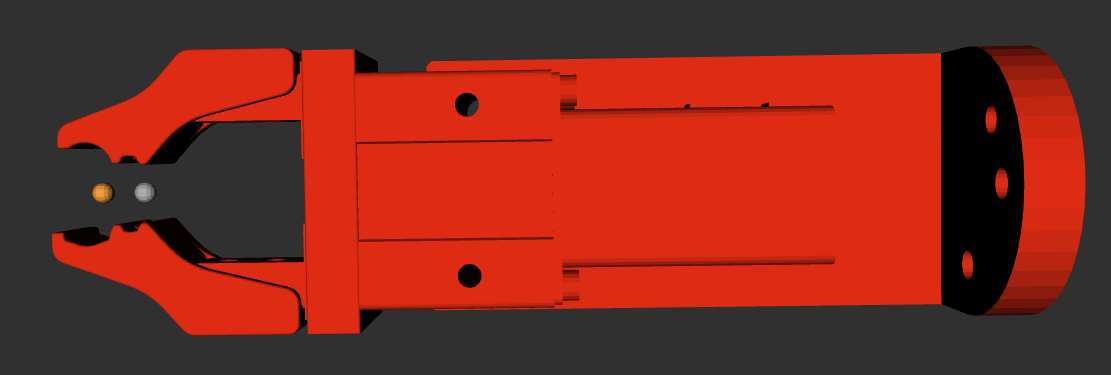
\includegraphics[width=0.8\textwidth]{greifer}
	\caption{Visualisierung der Greiferframes}
	\label{fig:Greifer}
\end{figure}

\subsection{Unterbau}
Im xacro der Anlage wird nur das Visuelle Modell der Anlage geladen, da ansonsten die Ladezeiten beim starten der move\_group extrem hoch sind und diese oft abstürzt. Das Kollisionsobjekt wird sobald die move\_group gestartet ist eingebunden (siehe Abschnitt \ref{sec:penAssembly}). Falls bei einem xacro kein Kollisionsobjekt definiert wird, wird automatisch der visuelle Teil auch für die Kollisionsberechnung verwendet. Aus diesem Grund wurde als Kollisionsobjekt eine Kugel mit Radius $0.1\;mm$ definiert und so positioniert, das diese sich in der Base des Roboters befindet.
\begin{code}
	\begin{minted}{xml}
<collision>
	<origin rpy="0 0 0" xyz="0 0 0.005" />
	<geometry>
		<sphere radius="0.0001" />
	</geometry>
</collision>	
	\end{minted}
	\vspace{-15pt}
	\caption{Dummy Kollisionsobjekt der Anlage}
	\label{code:dummyAnlage}
\end{code}

\subsection{Gesammte Anlage}
Die generierten Einzelteile der Anlage werden anschliessend in einem einzelnen .xacro-File eingebunden, als Ankerpunkt für den Greifer, Roboter und den Unterbau wird ein leerer Link mit dem Namen World definiert.
\begin{code}
	\begin{minted}{xml}
<?xml version="1.0" ?>
	<robot name="cell_tx260l" xmlns:xacro="https://ros.org/wiki/xacro">
	<xacro:include filename="$(find cell_support)/urdf/gripper_definition.xacro"/>
	<xacro:include filename="$(find cell_support)/urdf/unterbau.xacro" />
	<xacro:include filename="$(find staubli_tx260l_support)/urdf/tx260l_macro.xacro"/>
	
	<link name="world"/>
	
	<!-- init robots -->
	<xacro:gripper_definition prefix="" />
	<xacro:unterbau prefix=""/>
	<xacro:staubli_tx260l prefix="" />
	
	<!-- Joints -->
	<joint name="world_to_tx260l" type="fixed">
		<parent link="world" />
		<child link="base_link"/>
		<origin xyz="0 0 0" rpy="0 0 0"/>
	</joint>  
	<joint name="world_to_unterbau" type="fixed">
		<parent link="world" />
		<child link="unterbau_base"/>
		<origin xyz="0 0 0" rpy="0 0 0"/>
	</joint> 
	<joint name="tool0_to_gripper" type="fixed">
		<parent link="tool0" />
		<child link="gripper_base" />
		<origin xyz="0 0 0" rpy="0 1.57 0" />
	</joint>
</robot>	
	\end{minted}
	\vspace{-10pt}
	\caption{.xacro-File der gesammten Anlage}
	\label{code:xacroAnlage}
\end{code}

\section{MoveIt! Konfiguration}\label{sec:MoveitSetup}
Das erstellen der MoveIt! Konfiguration muss für alle Roboter welche in der Anlage eingebaut werden sollen durchgeführt werden, die Einstellungen sind dabei für alle Roboter identisch. Nachfolgend sind alle vorgenommenen Einstellungen aufgelistet, welche im Setup Assistant vorgenommen wurden.\\
\paragraph{Self-Collisions}
Als erstes wird der Setup Assistant gestartet und das .xacro-File geladen, anschliessend kann im Tab Self-Collisions die Kollisionsmatrix erstellt. Dabei kann die Sampling Density auf High gestellt werden.
\paragraph{Virtual Joints} Als nächstes muss ein Virtual Joint definiert werden, dieses verbindet die simulierte Welt mit dem geladenen .xacro-File, als Child Link wird dabei der definierte Ankerlink World gewählt, das Parent Frame ist World, und der Joint Type ist fixed. Als Name wurde hier jeweils FixedBase gewählt, dieser kann jedoch frei gewählt werden.
\paragraph{Planning Groups}
Es müssen zwei Planungsgruppen erstellt werden, eine small\_gripper und eine gripper. Je eine für die unterschiedlichen Frames des Greifers. Beide Planungsgruppen werden als Kinematische Kette definiert mit Start beim base\_link des Roboters und als Ende das entsprechende Frame. Als Kinematischersolver kann aus drei Standard Solvern gewählt werden und dem zusätzlich installierten Solver von TRACLabs. Für alle Roboter und Kinematischen Ketten wird der Solver 'trac\_ik\_kinematics' von TracLab gewählt. Es hat sich in Tests gezeigt, dass der Solver von TRACLabs, im Vergleich zu den Standardsolvern, fast immer eine Lösung findet. Die Einstellungswerte des Solvers wurde dabei auf den Standartwerten belassen.
\paragraph{Robot Poses}
Im Tab Robot Poses können Positionen des Roboters definiert werden, welche im \gls{GUI} der move\_group direkt ausgewählt werden können. Hier wurden zwei Posen definiert, eine mit allen Gelenken in Nullposition und eine Warteposition. 
\paragraph{End Effectors}
Im Abschnitt End Effectors muss nichts eingestellt werden. Hier würden Endeffektoren, die von der move\_group gesteuert werden definiert werden.
\paragraph{Passive Joints}
Im Abschnitt Passive Joints muss nichts angepasst werden. Hier würden Gelenke definiert werden, welche nicht angetrieben sind.
\paragraph{Author Information}
Es müssen Namen und Emailadressen des Erstellers diese Packages angegeben werden, ansonsten lässt sich das Setup nicht beenden.
\paragraph{Configuration Files}
In diesem Setup muss der Pfad angegeben werden, wo das Package abgespeichert werden soll, der Paketname muss, gemäss den ROS-Konventionen, dabei auf

'\_moveit\_config' enden. % das muss so sein!!


\section{Anpassungen ROS-I}
Für ROS-Industrial müssen nach dem Erstellen des Packages mit dem Setup Assistant einige Dateien hinzugefügt, respektive abgeändert werden. 
\paragraph{controllers.yaml}
Als erstes muss die Datei 'controllers.yaml' im config Ordner erzeugt werden, welche den ROS-Node 'Controller Manager' zur Verfügung stellt der von der move\_group gebraucht wird. Die Datei ist für alle Roboter gleich. Es muss jedoch beachtet werden, dass die Bezeichnungen der Gelenke mit deren des Roboters übereinstimmen müssen. 
\begin{code}
	\begin{minted}{yaml}
controller_list:
      - name: ""
      action_ns: joint_trajectory_action
      type: FollowJointTrajectory
      joints: [joint_1, joint_2, joint_3, joint_4, joint_5, joint_6]
	\end{minted}
	\vspace{-15pt}
	\caption{controller.yaml}
	\label{code:controller}
\end{code}

\paragraph{controller\_manager.launch}
Das .launch-File um den Controller zu starten ist nach dem Erstellen der Konfiguration zwar vorhanden jedoch ist es leer. Das File muss für jeden Roboter spezifisch angepasst werden. Es benötigt den Pfad zum jeweiligen 'controller.yaml'. Nachfolgend eine Vorlage, bei welcher der Teil in den eckigen Klammern ergänzt werden muss.
\begin{code}
	\begin{minted}{xml}
<launch>
	<arg name="moveit_controller_manager"
	  default="moveit_simple_controller_manager/MoveItSimpleControllerManager"/>
	<param name="moveit_controller_manager"
	      value="$(arg moveit_controller_manager)"/>	
	<rosparam file="$(find [robot_moveit_config])/config/controllers.yaml"/>
</launch>	
	\end{minted}
	\vspace{-15pt}
	\caption{Vorlage '..controller\_manager.launch'}
	\label{code:controllerManager}
\end{code}

\paragraph{moveit\_planning\_execution.launch}
Als letztes muss ein .launch-File erzeugt werden, welches alle für ROS-I benötigten Nodes startet. Eine Vorlage dieses Files ist im Anhang unter \ref{Anhang:MoveitVorlage} zu finden. Auch in diesem File müssen einige Teile spezifisch auf die Roboter angepasst werden. 
\section{ROS}
Damit ROS-I mit dem Roboter Kommunizieren kann muss auf den Robotersteuerungen Anpassungen vorgenommen werden.
\paragraph{ABB IRB 120}
Für den ABB IRB120 ist es nötig einen ROS Server auf dem Controller des Roboters zu installieren. Es müssen einige neue Tasks auf der Steuerung erstellt werden sowie ein RAPID-Programm auf die Steuerung geladen werden. Eine sehr detaillierte Anleitung dazu ist auf den ROS-Wikipages\footnote{\url{http://wiki.ros.org/abb/Tutorials/InstallServer}} zu finden.

\paragraph{Stäubli TX2-60l}
Da der Stäubli Roboter bei Abschluss dieser Arbeit noch nicht geliefert wurde können keine konkreten Angaben über die nötigen Anpassungen auf dem Controllers gemacht werden. Es stehen Driver für die Steuerung CS8 zur Verfügung, gemäss Informationen von Stäubli wird der Roboter mit einer Steuerung vom Typ CS9 geliefert. Bei Erhalt des Roboters und der Steuerung müssen diese mit ROS getestet werden und allenfalls der Server für die Steuerung angepasst werden. Die benötigten Files sowie eine Anleitung in Form eines Readmes befinden sich im Ordner /staubli\_expermintal/staubli\_val3\_driver.

\paragraph{Universal UR3}
Für den Universal Robot UR3 muss keine zusätzliche Software installiert werden, da Universal Robot Standardmässig auf ihrer Steuerung bereits ROS Messages verarbeiten kann. Somit genügt es auf der Robotersteuerung das Netzwerk zu konfigurieren respektive kontrollieren ob dieses eingeschaltet ist. 
\chapter{Implementierung Montage}
In diesem Kapitel wird auf die Implementierung aller notwendiger Softwarekomponenten eingegangen, damit im Industriedemonstrator Kugelschreiber montiert werden können. 
\section{Grundüberlegungen}
Der Roboter muss fähig sein einem Montageablauf zu folgen, um Kugelschreiber montieren zu können. Dieser wird in einem eigenen Package cell\_core implementiert. Dieses Package erzeugt die move\_group und kann Kollisionsobjekte in der Planungsszene generieren. Ein zweites Package ist für die Ansteuerung der SMC Aktuatoren zuständig. Dieses Package smc\_grippers ist die Schnittstelle zwischen der ROS-Kommunikation und der Kommunikation über EtherCAT. Für die Schnittstelle zur restlichen Anlage steht der in Abschnitt \ref{sec:SWschnittstellen} bereits erwähnte HTTP-Server zur Verfügung. Dieser befindet sich im Package http\_server.
\begin{figure}[H]
	\centering
	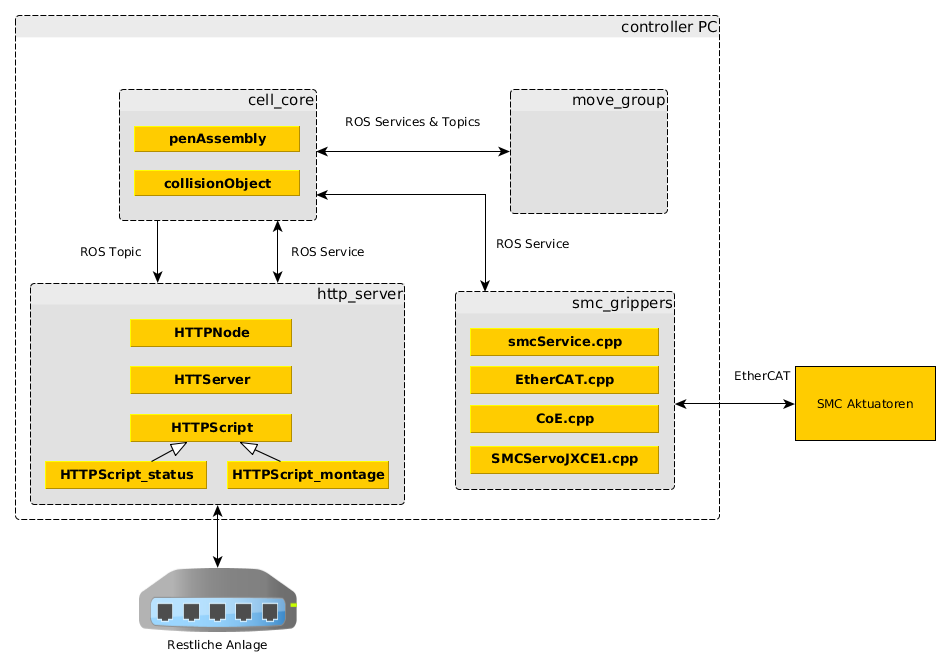
\includegraphics[width=0.95\textwidth]{uebersicht}
	\caption{Übersicht Packages und Kommunikation}
	\label{fig:Uebersicht}
\end{figure}

\section{cell\_core}
Das Package cell\_core ist das Kernelement der Implementierung von ROS. Das Package konstruiert die move\_group und kommuniziert anschliessend mit derselben um den momentan in der Anlage verbauten Roboter in Bewegung zu bringen. Das Package besteht aus einem Node 'penAssembly' und einer Klasse 'collisionAdder'. Das Package publiziert beim ROS-Master zwei Services und ein Topic, mit welchen es möglich ist mit dem Package zu kommunizieren.

\subsection{Topics}
Der Node publiziert regelmässig($10\;Hz$) den momentanen Anlagenstatus auf dem Topic /penAssembly/status. Die Publizierte Nachricht enthält die zwei booleschen Variablen idle und error. Welche je nach Zustand der Anlage gesetzt werden.

\subsection{Services}
Das Package cell\_core bietet zwei Services an, der erste Service startet den Zusammenbau eines Kugelschreibers. Der zweite Service ermöglicht es den Roboter an einen bestimmten Punkt und Orientierung zu bewegen.
\paragraph{moveRobotToPose}
Zum jetzigen Stand der Arbeit registriert sich bei diesem Service kein Node. Der Service wurde nur gebraucht um den Roboter über die Konsole mithilfe von\\
\mintinline{bash}{$ rosservice call /penAssembly/moveRobotToPose "x: ,y: ,z: ,oW: ,oX: ,oY : ,oZ: "} %$
zu einer bestimmten Position und Orientierung zu bewegen. Die Methode beachtet bei der Planung der Bewegung Kollisionsobjekte. Der Service Antwortet mit einem Boolean ob die Position erreicht wurde (true) oder nicht (false). Zum Aufrufen des Services müssen die Koordinaten sowie die Orientierung angegeben werden. Der Service ruft die Methode 'moveRobotCallback' auf.
\paragraph{montage\_service}
Der Service montage\_service ermöglicht es den Start der Montage auszulösen. Dabei muss der Nachricht der Offset der Wagen in Metern, sowie die gewünschte Ausgabestelle für den fertig montierten Kugelschreiber mitgegeben werden. Momentan ist die Ausgabe an verschiedene Stellen nur implementiert es existieren in der Anlage aber noch keine effektiven Ausgabestellen.
\begin{figure} [h!]
	\begin{minipage}[h]{0,49\textwidth}
		\begin{code}
			\begin{minted}{bash}
			#request
			float64 x
			float64 y
			float64 z
			float64 oW
			float64 oX
			float64 oY
			float64 oZ
			---
			#response
			bool status
			\end{minted}
			\vspace{-10pt}
			\caption{moveRobotToPose Message}
			\label{code:moveRobotMessage}
		\end{code}
	\end{minipage}
	\begin{minipage}[h]{0,49\textwidth}
		\begin{code}
			\begin{minted}{bash}
			#request
			float64 Offset
			int64 Ausgabestelle
			---
			#response
			int64 status			
			\end{minted}
			\vspace{-10pt}
			\caption{montage\_service Message}
			\label{code:montageMessage}
		\end{code}
	\end{minipage}
\end{figure}

\subsection{penAssembly} \label{sec:penAssembly}
\paragraph{Initialisierung}
Beim starten des penAssembly Nodes wird als erstes ROS initialisiert und anschliessend ein asynchroner Spinner gestartet. Der asynchrone Spinner ist nötig, damit bei aktiver Planung von Trajektorien andere Anfragen immer noch verarbeitet werden können. Anschliessend wird die move\_group gestartet und initialisiert, gefolgt vom Publizieren der beiden Services und des Topics. Als letztes wird ein Objekt der Klasse collisionObject erstellt und das Kollisionsobjekt der Anlage auf dem planning\_interface publiziert. Wenn dieses Setup durchgeführt wurde wechselt der Node in einen Endlosloop und publiziert mit einer Frequenz von $10\;Hz$ den Status der Anlage. Gleichzeitig wird auf den beiden publizierten Topics auf eine Anfrage gewartet.
\begin{code}
	\begin{minted}{cpp}
int main(int argc, char **argv)
{
	ros::init(argc, argv, "penAssembly");
	ros::NodeHandle nh;
	ros::AsyncSpinner spinner(0); // Define Multithreadedspinner
	spinner.start();

	// Define MoveGroup and PlanningSceneInterface
	group.reset(new moveit::planning_interface::MoveGroupInterface("gripper"));
	//group->setPlannerId("RRTConnect");
	group->setEndEffectorLink("grasping_frame");
	group->setPlanningTime(1.5);
	group->setGoalJointTolerance(0.0001);
	group->setNumPlanningAttempts(3);
	group->setGoalOrientationTolerance(0.0001);
	group->setMaxVelocityScalingFactor(0.1);

	// Advertise Services at ROS-Master
	ros::ServiceServer service = nh.advertiseService("/penAssembly/montage_service", montageCallback);
	ros::ServiceServer moveservice = nh.advertiseService("/penAssembly/moveRobotToPose", moveRobotCallback);
	ROS_INFO("Service rdy!");

	// Publish the Status updater
	ros::Publisher penAssembly_pub = nh.advertise<cell_core::status_msg>("/penAssembly/status", 1000);

	sleep(15); // to make sure move_group is up
	collisionObject coAdder;
	coAdder.addCell(group);
	sleep(10);	// only used because the large model takes some time to load

	ROS_INFO("Node Ready!");
	// Publish the State of the Assembly
	ros::Rate loop_rate(10); //Freq of 10 Hz
	while (ros::ok()) //aslong as node is alive
		{
			cell_core::status_msg msg;
			msg.idle = idle_;
			msg.error = error_;
			penAssembly_pub.publish(msg);
			loop_rate.sleep();
		}
}	
	\end{minted}
	\caption{Initialisierung penAssembly Node}
	\label{code:initPenAssembly}
\end{code}

\subsubsection{Methoden}
Der Node bietet mehrere Methoden, zwei der Methoden werden durch die Services aufgerufen, die restlichen Methoden werden durch diese beiden Callbackmethoden aufgerufen. Alle in penAssembly.cpp implementierten Methoden ermöglichen es dem Roboter sich auf eine bestimmte Art und Weise zu bewegen. 

\paragraph{montageCallback}
Die Methode montageCallback wird vom Service montage\_service aufgerufen. Die Methode überprüft zu Beginn, ob die mitgegebenen Werte korrekt sind und ob die Anlage sich im idle-Modus befindet. Falls die Kriterien erfüllt sind startet die Anlage die Montage eines Kugelschreibers, ansonsten wird kein Kugelschreiber montiert und ein Fehler zurückgegeben. Innerhalb der Methode ist der Ablauf für die Montage des Kugelschreibers definiert. Der Roboter fährt jeweils mit freier Trajektorienplanung an ein Offset Punkt vor der eigentlichen Pose. Anschliessend wird der restliche Weg mit einem linearen Fahrbefehl gefahren. 

\paragraph{initPoses}
Die Methode init Poses wird bei jedem Start eines Montage Prozesses aufgerufen, diese Initialisiert alle für die Montage benötigten Posen des Roboters. Ihr wird der Offset aus dem Servicecall mitgegeben, damit die Position des Schlittens korrigiert werden kann.

\paragraph{moveLinear}
Diese Methode bewegt den Roboter auf einer geraden Linie zwischen zwei Punkten. Der Startpunkt entspricht dabei immer der momentanen Position des Roboters, als Endpunkt kann entweder der Fahrweg von Startpunkt zu Zielpunkt in Metern in x,y,z mitgegeben werden, oder eine Pose zu welcher gefahren werden soll. Die Methode benötigt zudem den Plan des MoveGroupInterfaces.
Die Trajektorie zwischen dem Start- und Endpunkt wird mithilfe der Methode computeCartesianPath berechnet, welche Teil der move\_group ist. Der Trajektorie wird nur ausgeführt, falls der Planner mehr als 90\;\% des vorgegebenen Weges einhalten kann. Falls dies der Fall ist gibt die Methode true zurück.
\begin{code}
	\begin{minted}{cpp}
bool moveLinear(double x, double y, double z, moveit::planning_interface::MoveGroupInterface::Plan &plan)
{
    std::vector<geometry_msgs::Pose> waypoints_tool;
    // Getting the current pose
    geometry_msgs::PoseStamped tempStampPose = group->getCurrentPose(group->getEndEffectorLink());
    geometry_msgs::Pose test_pose = tempStampPose.pose;
	// Defining Endpose
    test_pose.position.x += x;
    test_pose.position.y += y;
    test_pose.position.z += z;
    waypoints_tool.push_back(test_pose);

    moveit_msgs::RobotTrajectory trajectory_msg;
    double fraction = group->computeCartesianPath(waypoints_tool,
                                                  0.001, //eef_step
                                                  5,     // jump_threshold
                                                  trajectory_msg, 
                                                  true); //avoid collisions
    plan.trajectory_ = trajectory_msg;
    ROS_INFO("Visualizing Cartesian Path (%2f%% acheived)", fraction * 100.0);
    if (fraction >= 0.90)
    {
        group->execute(plan);
        return 1;
    }
    else
    {
        return 0;
    }
    return -1;
}
	
	\end{minted}
	\vspace{-10pt}
	\caption{moveLinear mit x,y,z Offset}
	\label{code:moveLinear}
\end{code}

\paragraph{movePen}
Die Methode movePen wird gebraucht um den Kugelschreiber von der 45\;\textdegree Lage in die Senkrechte Position aufzurichten. 

\paragraph{rotateZ}
Die Methode rotateZ wird aufgerufen um den Kugelschreiber mit dem Werkzeuge auszurichten. Sie ist die einzige Methode, welche anstatt auf Positionen zu Planen direkt auf Gelenkwinkel plant. Der Methode muss ein Winkel in Radiant mitgegeben werden, um welchen sich die sechste Achse in positiver Richtung drehen soll.
\begin{code}
	\begin{minted}[breakanywhere]{cpp}
void rotateZ(moveit::planning_interface::MoveGroupInterface::Plan &plan, double angle)
{
	std::vector<double> group_variable_values;
	// Saves the current Joint values in the vector group_variable_values
	group->getCurrentState()->copyJointGroupPositions(group->getCurrentState()->getRobotModel()->getJointModelGroup(group->getName()), group_variable_values);
	// Defining goal JointValue of joint6
	group_variable_values[5] += angle;
	group->setJointValueTarget(group_variable_values);
	// plan and execute
	group->plan(plan);
	group->execute(plan);
}
	\end{minted}
\vspace{-10pt}
\caption{Methode rotateZ}
\label{code:methRotz}
\end{code}

\paragraph{moveToPose}
Die Methode moveToPose bewegt den Roboter an die angegebene Pose, es ist möglich der Methode einen Offset in x,y und z mitzugeben. Falls der Planer beim ersten versuch keine Lösung findet wird die Planungszeit auf $10\;s$ erhöht und ein neuer Planungsversuch gestartet. Falls immer noch keine Lösung für die Bewegung gefunden wird gibt die Methode false zurück.

\subsection{collisionAdder}
Die Klasse collisionAdder ermögtlicht es Kollisionsobjekte in die Planungsszene zu laden, dazu bietet sie vier Methoden an.
\paragraph{addCell} Die Methode addCell wird kurz nach dem erstellen des Objekts beim Initialisieren des Nodes aufgerufen. Sie fügt der Planungsszene das Kollisionsmodell der Anlage hinzu, welches direkt aus dem .stl-File generiert wird. 
\begin{code}
	\begin{minted}{cpp}
void collisionObject::addCell(boost::shared_ptr<moveit::planning_interface::MoveGroupInterface> &group)
{
    // Generating Collision object from Mesh
    Eigen::Vector3d scaling_vector(0.001, 0.001, 0.001); // Scaling Vector
    moveit_msgs::CollisionObject co;
    co.header.frame_id = group->getPlanningFrame();
    co.id = "WorkCell";
    shapes::Mesh *m = shapes::createMeshFromResource("package://cell_support/meshes/1000_Anlage_collision.stl", scaling_vector);
    ROS_INFO("Mesh Loaded");

    shape_msgs::Mesh mesh;
    shapes::ShapeMsg mesh_msg;
    shapes::constructMsgFromShape(m, mesh_msg);
    mesh = boost::get<shape_msgs::Mesh>(mesh_msg);

    // Define position and orientation
    co.meshes.resize(1);
    co.mesh_poses.resize(1);
    co.meshes[0] = mesh;
    co.mesh_poses[0].position.x = -1.075;
    co.mesh_poses[0].position.y = 0.023;
    co.mesh_poses[0].position.z = -0.021;
    co.mesh_poses[0].orientation.w = 0.707;
    co.mesh_poses[0].orientation.x = 0.0;
    co.mesh_poses[0].orientation.y = 0.0;
    co.mesh_poses[0].orientation.z = 0.707;

    // Push onto vector and publish it on the szene
    co.meshes.push_back(mesh);
    co.mesh_poses.push_back(co.mesh_poses[0]);
    co.operation = co.ADD;
    std::vector<moveit_msgs::CollisionObject> collision_objects;
    collision_objects.push_back(co);
    planning_scene_interface.addCollisionObjects(collision_objects);
    return;
}

	\end{minted}
\vspace{-10pt}
\caption{addCell Methode}
\label{code:addCell}
\end{code}

\paragraph{addBody}
Die Methode addBody publiziert einen Kollisionskörper am momentan aktiven Planningframe des Roboters und befestigt diesen direkt daran. Die Methode besitzt ein Switchstatement, welches einen Übergabewert auswertet. Mit diesem kann zwischen der vorderen Hülle (1) dem Deckel (2), der Miene (3) und dem Werkzeug (4) ausgewählt werden. Die Kollisionskörper werden wie bei der Methode addCell direkt aus den .stl-Files der Teile erstellt. 

\paragraph{detatchBody}
Diese Methode entfernt ein zuvor publiziertes Kollisonsobjekt vom Roboter, entfernt es jedoch noch nicht aus der Plannungsumgebung. Auch hier können die Objekte wieder über den übergebenen Integer ausgewählt werden.

\paragraph{removeBody}
Die Methode entfernt ein sich in der Planungsszene befindendes Objekt ganz. Die Methode benötigt die selben Übergabewerte wie die beiden vorhergegangenen Methoden.

\subsection{launch}
Das Package enthält zwei launch-Files, das Erste startet alle benötigten Nodes für den Industriedemonstrator, verbindet sich aber nicht mit einem angeschlossenen Roboter. Das andere .launch-File startet auch alle benötigten Nodes, versucht aber zudem eine Verbindung mit dem angeschlossenen Roboter herzustellen (momentan ABB IRB120).
Es wurden auch launch-files für den Stäubliroboter generiert, bei diesen konnte jedoch nicht getestet werden ob sie eine Verbindung mit dem Roboter herstellen, da der Roboter noch nicht geliefert wurde.

\section{http\_server}
Der HTTP-Server basiert auf dem im SVN-Repository \url{https://triest.zhaw.ch/svn/iio/} vorhandenen Sourcecode. Es wurde zusätzlich ein ROS Node erstellt, welcher die für den Betrieb des HTTP-Servers nötigen Objekte generiert. Der Node erstellt zwei unterschiedliche Server auf den Ports 8080 und 8081, auf dem Port 8080 kann die Montage eines Kugelschreibers ausgelöst werden. Dazu muss die folgende URL mit den entsprechenden Werten aufgerufen werden:\\
\url{http://160.85.95.166:8080/cgi-bin/montage?offset=0.0\&ausgabestelle=1}\\
Der Offset muss in Metern angegeben werden wobei positive Zahlen einen Offset in Fahrtrichtung der Wagen entsprechen.\\

Mit dem Webserver auf Port 8081 kann der Status des Roboters abgefragt werden, dazu kann die folgende URL aufgerufen werden:\\
\url{http://160.85.95.166:8080/cgi-bin/status}

Bei beiden Aufrufen ist allenfalls die IP-Adresse zu ändern.

\begin{code}
	\begin{minted}{cpp}
#include <http_server/HTTPNode.h>

int main(int argc, char **argv)
{
    ros::init(argc, argv, "HTTP_server");
    ros::NodeHandle nh;
    ros::AsyncSpinner spinner(2); // Define Multithreadedspinner
    spinner.start();

    HTTPServer *httpServer = new HTTPServer(8080);
    HTTPServer *httpServer2 = new HTTPServer(8081);
    httpServer->start();
    httpServer2->start();
    httpServer->add("montage", new HTTPScript_montage());
    httpServer2->add("status", new HTTPScript_status());

    ROS_INFO("Http-Server is running!");

    ros::waitForShutdown();
}
	\end{minted}
\vspace{-10pt}
\caption{Main des HTTP-Servers}
\label{code:httpMain}
\end{code}
\subsection{launch}
Der Webserver kann über das launch-File 'httpNode.launch' gestartet werden, das launchfile Startet im falle eines Absturzes des HTTP-Nodes diesen direkt neu.

\section{smc\_grippers}
Die Controller für die SMC Aktuatoren müssen über EtherCAT angesteuert werden. Durch die ROS Community sind einige Packages vorhanden, welche dazu gedacht sind EtherCAT Geräte anzusteuern. Diese basieren in der Regel entweder auf dem \gls{SOEM} der OpenEtherCAT Society, oder auf dem EtherCAT Treiber des PR2 von Willow Garage. Es wurde mit mehreren dieser verfügbaren Packete versucht eine erfolgreiche Kommunikation mit den EtherCAT Kontrollern von SMC aufzubauen. Diese Versuche blieben jedoch erfolglos. Aus diesem Grund wurde durch Herrn Dr. Marcel Honegger ein Treiber für die EtherCAT Kontroller von SMC geschrieben. Diese Sourefiles wurden anschliessend in ein ROS Node eingebunden, welcher für jeden Aktuator von SMC einen eigenen Service anbietet.\\
\begin{code}
	\begin{minted}{cpp}
bool smcService::gripperCallback(smc_grippers::gripper_service::Request &req, smc_grippers::gripper_service::Response &res)
{
    gripper->enable();
    int pos = req.position;
    gripper->setTargetPosition(pos);
    gripper->disable();
    return 1;
}
	\end{minted}
\vspace{-10pt}
\caption{Callbackmethode des Greifers}
\label{code:CallbackGripper}
\end{code}

Im momentanen Stand der Anlage ist noch keine Kommunikation mit den Kontrollern von SMC möglich, da es vom Linux PC nicht möglich ist, dass die Slaves in den EtherCAT status Operational wechseln. 

\subsection{Services} %TODO: Services anpassen und SMC Teil programmieren.
Die drei Services sind identisch aufgebaut und benötigen alle nur die gewünschte Position in Millimeter. Die Services antworten immer mit true, ausser die Services sind nicht erreichbar.

\subsection{launch}
Der SMC Node kann mithife des launch-File 'smcService.launch' gestartet werden.


%!TEX root = ../doc.tex
\chapter{Resultate}
\label{sec:Resultate}
\section{Simulation Montageaufgabe}
Die Montageaufgabe kann in RVIZ simuliert werden. Im momentanen Stand der Arbeit kann es Vorkommen, dass keine Lösungen für das Anfahren von gewissen Positionen gefunden werden.

\section{Umsetzung Montageaufgabe}
Die Montageaufgabe konnte in der Simulation mit den von ROS zur Verfügung gestellten Tools implementiert werden. Da die beiden Bachelorstudenten einige Teile für die Montagezelle falsch gezeichnet haben und diese somit nicht montiert werden konnten mussten die Teile neu modelliert und anschliessend 3D-gedruckt werden. Zusätzlich kamen Probleme mit der Genauigkeit der CAD-Modelle hinzu und das mit dem ABB IRB120 in der vorgesehenen Konfiguration der Anlage nicht alle Montagepunkte erreicht werden konnten. All diese Faktoren führten dazu, dass für ausführliche Tests der Simulation sowie realen Anlage die Zeit fehlte.
Der Komplette Sourecode sowie die erstellten Packages und CAD-Files sind auf dem pool unter:\url{//shared.zhaw.ch/pools/t/T-IMS-SmartPro/Projekt/ROS-Industrial} zu finden.
\section{Portierung Montageaufgabe}
Da der Staubli Roboter erst nach Abschluss der vorliegenden Arbeit geliefert wird wurde die Montageaufgabe auf dem Roboter von ABB vom Typ IRB120 realisiert. Über eine mögliche Portierung der Montageaufgabe auf den Roboter von Stäubli können keine fundierten Resultate abgegeben werden. Es konnte ein Driver für den Controller vorbereitet werden, ob dieser auf der echten Steuerung wirklich funktioniert muss nach Erhalt des Roboters geklärt werden.

\section{Evaluation ROS-Industrial}
ROS und ROS-Industrial sind zwei extrem mächtige Tools, sie haben ihre Vorteile aber auch ihre Nachteile. In diesem Abschnitt wird auf die wichtigsten Eigenschaften von ROS-I eingegangen. 
\subsection{Verfügbarkeit von Paketen}
ROS und ROS-Industrial werden zu einem sehr grossen Teil durch die Community erweitert und gewartet. Auf diversen Repositorys verteilt befinden sich eine sehr grosse Anzahl an Packages, welche diverse Funktionen und/oder Bibliotheken enthalten. Viele dieser Packages werden einigermassen gut gewartet und aktualisiert, fast genau so viele Packages sind jedoch fast verwahrlost.\\
Oft wird zum Implementieren einer Funktion auf diese grosse Anzahl an Funktionen und Bibliotheken zurückgegriffen, oder aber es werden andere OpenSource Ressourcen eingebunden wie zum Beispiel die OMPL. Dies bietet einige Vor- und Nachteile, einerseits sind viele Probleme schon bereits irgendwo entstanden und es bestehen Lösungen oder zumindest Lösungsansätze. Die Funktion, Stabilität und Wartung solcher Pakete ist jedoch überhaupt nicht gewährleistet und muss allenfalls selbst in die Hand genommen werden.

\subsection{Zuverlässigkeit und Stabilität}
Die von ROS-Industrial angebotenen Funktionen sind alle relativ zuverlässig, ausser der Descrates Planer. Dieser konnte selten eine vernünftige Lösung für die gestellten Trajektorienbahnen finden und stürzte oft ab. Die Nodes welche generiert werden sind in sich auch stabil und bei einem Absturz eines Nodes wird aufgrund der Systemarchitektur von ROS ein kompletter Systemausfall verhindert. Trotzdem muss der Node anschliessend neu gestartet werden, was in einem Industriedemonstrator welcher später an einer Messe laufen soll nicht sehr von Vorteil ist. 

\subsection{Support}
Der Support von ROS-Industrial setzt rein auf die Foren und Wikipages. Diese Foren und Wikipages sind Voll mit Informationen und viele Probleme welche während dieser Arbeit entstanden sind konnten über diese relativ schnell gelöst werden. Trotzdem kann es vorkommen, dass ein Problem entsteht bei welchem weder die Wikipages oder die Foren helfen können. In diesem Fall ist 

\subsection{Empfehlung ROS-I}
ROS-Industrial bietet viele Funktionen an, welche für die Industrie gebraucht werden, die sehr ausgereift und durchdacht sind. Gleichzeitig scheint es aber bei einigen Teilen noch in den Kinderschuhen zu stecken. Im momentan scheint ROS-Industrial für die Anwendung im Industriedemonstrator nicht geeignet zu sein. Die Implementierung der Montageaufgabe ist zwar nicht ausserordentlich Komplex, jedoch konnten einige Probleme nicht oder nur mit behelfsmässigen Patches gelöst werden. Eine realisierung der Montageaufgabe mithilfe der vom Hersteller zur Verfügung gestellten Tools scheint hier wesentlich schneller und vor allem stabiler zu Funktionieren.\\

ROS-Industrial ist interessant für Anwendungen in welchen sich die Umgebungen ändern und diese mit Sensoren oder Kameras überwacht werden können. Dort kann ROS durch seine dynamische Bahnplanung und direkte Verarbeitung von Sensor- und Kameradaten punkten. Ein weiterer Vorteil von ROS ist die Freiheit mit einer Applikation unterschiedliche Robotertypen anzusteuern, somit wäre ROS sicherlich in einer Anlage mit mehreren unterschiedlichen Robotern geeignet.

\section{Probleme und offene Punkte}
\subsection{SMC Aktuatoren}
Beim Momentanen Stand der Arbeit konnte keine Kommunikation über EtherCAT mit den Aktuatoren von SMC hergestellt werden. Die Kommunikation über EtherCat mit den Kontrollern Funktioniert zwar, jedoch weigern sich die Kontroller vom EtherCAT Staus "Safe Operational" in den Status "Operational" zu wechseln. Aus diesem Grund kann von ROS aus im Moment die Aktuatoren nicht angesteuert werden. Aus diesem Grund konnten die Greiferpositionen noch nicht bestimmt werden und es konnten somit auch keine Kugelschreiber in der Anlage zusammengebaut werden.
 
\subsection{Crash Nodes}
Es kann vorkommen, dass die move\_group, RVIZ oder ein anderer Node sich während der Bahnplanung oder auch sonst \textgravedbl aufhängt\textacutedbl. Bis zur Abgabe dieser Arbeit konnte die Ursache für dieses Vorkommen nicht eindeutig ermittelt werden.

\subsection{Fahrgeschwindigkeit und Aborts}
ROS berechnet aufgrund der maximalen Gelenkgeschwindigkeiten und des zu verfahrenden Weges die Zeit die es Braucht um die Ziel Position zu erreichen. Diese Zeit wird mit einem Faktor (Standardwert 1.2) multipliziert und ergibt die maximal erlaubte Plannungszeit. Falls diese vom Roboter überschritten wird wird durch die move\_group das Ausführen der Trajektorie abgebrochen. Dies kommt beim ABB IRB120 in der Simulation nicht vor, jedoch kann es auf dem echten Roboter dazu kommen. Eine erhöhung des Faktors oder gar eine Deaktivierung dieser Funktion scheinen keine Auswirkungen auf dieses Abbruchkriterium zu haben.

%!TEX root = ../doc.tex
\chapter{Diskussion und Ausblick}
\label{sec:DiskussionUndAusblick}

\section{Erreichung der Ziele}
Nicht alle gesteckten Ziele für diese Arbeit konnten erreicht werden. Es konnte eine Arbeitsumgebung für ROS und ROS-Industrial eingerichtet werden, mit welcher die Implementierung der Montageaufgabe in den Industrie 4.0 Demonstrator durchgeführt werden konnte. Zur Implementierung der Montageaufgabe musste ein sehr breites Basiswissen von ROS und ROS-Industrial angelegt werden. Dies ermöglicht nun fundierte Aussagen über die Möglichkeiten und Einschränkungen von ROS-Industrial machen zu können.\\

Aufgrund von falsch gezeichneten und falsch bestellten Teilen durch die beiden Bachelorstudenten, welche das mechanische Konzept der Anlage entwickelten, konnte erst kurz vor Abgabe erste Tests mit dem Greifer am Roboter gemacht werden. Dies nach hinten verschoben Testphase verunmöglichte es grosse Änderungen an der Implementation zu machen. Da zum Zeitpunkt der Abgabe der Arbeit die Aktuatoren von SMC noch nicht über EtherCAT angesteuert werden konnten, konnte noch kein Kugelschreiber montiert werden.

\section{Ausblick}
Sobald der Stäubli Roboter geliefert wird und dieser in der Anlage verbaut ist, kann die Implementierung von ROS-Industrial auf dessen Steuerung beginnen. Die Weiterführung von ROS-Industrial als Steuerung des Knickarmroboters ist meines erachtens nur sinvoll, falls in weiterer Zukunft an der ZHAW oder am IMS im Sinne der Forschung weiter mit ROS gearbeitet werden will. Oder falls die Komplexität der Montageaufgabe sich erhöht, weil zum Beispiel über Vision Sensoren Objekte im Arbeitsraum erkennt werden können und dynamisch umfahren werden sollen. \\
Ansonsten ist die Implementierung des momentanen Montageprozesses schneller und effizienter mit den bisherigen Robotertools.



%%% Verzeichnise %%%
\backmatter 
\label{sec:Verzeichnisse}
% Literaturverzeichnis
\bibliography{BibTeX/literatur}
\addcontentsline{toc}{chapter}{Literaturverzeichnis}


%%% Anhang %%%
\appendix
%!TEX root = ../doc.tex
\pagenumbering{Roman}

\appendix
\chapter{Anhang}
\label{sec:Anhang}
Im Anhang dieses Dokumentes befinden sich nur die in der Arbeit referenzierten Codeausschnitte sowie die Aufgabenstellung. Alle in dieser Arbeit generierten Files sind auf dem ZHAW pool unter: \url{//shared.zhaw.ch/pools/t/T-IMS-SmartPro/Projekt/ROS-Industrial} zu finden.

\section{Offizielle Aufgabenstellung}

\includepdf{anhang/Aufgabenstellung.pdf}

\newpage
\section{Sourcecodefiles}
\subsection{Vollständige CMakeLists}\label{Anhang:Cmakelists}
\inputminted[bgcolor=white]{cmake}{anhang/CMakeLists.txt}

\newpage
\subsection{moveit\_planning\_execution.launch}\label{Anhang:MoveitVorlage}
\inputminted[bgcolor=white]{xml}{anhang/moveit_planning_execution.launch}

\newpage
\subsection{tx260l\_macro.xacro} \label{Anhang:Staublixacro}
\inputminted[bgcolor=white]{xml}{anhang/tx260l_macro.xacro}




\end{document}
